% Template for PLoS
% Version 3.4 January 2017
\documentclass[10pt,letterpaper]{article}
\usepackage[top=0.85in,left=2.75in,footskip=0.75in]{geometry}

% amsmath and amssymb packages, useful for mathematical formulas and symbols
\usepackage{amsmath,amssymb}

% Use adjustwidth environment to exceed column width (see example table in text)
\usepackage{changepage}

% Use Unicode characters when possible
\usepackage[utf8x]{inputenc}

% textcomp package and marvosym package for additional characters
\usepackage{textcomp,marvosym}

% cite package, to clean up citations in the main text. Do not remove.
% \usepackage{cite}

% Use nameref to cite supporting information files (see Supporting Information section for more info)
\usepackage{nameref,hyperref}

% line numbers
\usepackage[right]{lineno}

% ligatures disabled
\usepackage{microtype}
\DisableLigatures[f]{encoding = *, family = * }

% color can be used to apply background shading to table cells only
\usepackage[table]{xcolor}

% array package and thick rules for tables
\usepackage{array}

% create "+" rule type for thick vertical lines
\newcolumntype{+}{!{\vrule width 2pt}}

% create \thickcline for thick horizontal lines of variable length
\newlength\savedwidth
\newcommand\thickcline[1]{%
  \noalign{\global\savedwidth\arrayrulewidth\global\arrayrulewidth 2pt}%
  \cline{#1}%
  \noalign{\vskip\arrayrulewidth}%
  \noalign{\global\arrayrulewidth\savedwidth}%
}

% \thickhline command for thick horizontal lines that span the table
\newcommand\thickhline{\noalign{\global\savedwidth\arrayrulewidth\global\arrayrulewidth 2pt}%
\hline
\noalign{\global\arrayrulewidth\savedwidth}}


% Remove comment for double spacing
%\usepackage{setspace} 
%\doublespacing

% Text layout
\raggedright
\setlength{\parindent}{0.5cm}
\textwidth 5.25in 
\textheight 8.75in

% Bold the 'Figure #' in the caption and separate it from the title/caption with a period
% Captions will be left justified
\usepackage[aboveskip=1pt,labelfont=bf,labelsep=period,justification=raggedright,singlelinecheck=off]{caption}
\renewcommand{\figurename}{Fig}

% Use the PLoS provided BiBTeX style
% \bibliographystyle{plos2015}

% Remove brackets from numbering in List of References
\makeatletter
\renewcommand{\@biblabel}[1]{\quad#1.}
\makeatother

% Leave date blank
\date{}

% Header and Footer with logo
\usepackage{lastpage,fancyhdr,graphicx}
\usepackage{epstopdf}
\pagestyle{myheadings}
\pagestyle{fancy}
\fancyhf{}
\setlength{\headheight}{27.023pt}
\lhead{
\includegraphics[width=2.0in]{PLOS-submission.eps}}
\rfoot{\thepage/\pageref{LastPage}}
\renewcommand{\footrule}{\hrule height 2pt \vspace{2mm}}
\fancyheadoffset[L]{2.25in}
\fancyfootoffset[L]{2.25in}
\lfoot{\sf PLOS}

%% Include all macros below
\newcommand{\lorem}{{\bf LOREM}}
\newcommand{\ipsum}{{\bf IPSUM}}

\usepackage{color}
\usepackage{fancyvrb}
\newcommand{\VerbBar}{|}
\newcommand{\VERB}{\Verb[commandchars=\\\{\}]}
\DefineVerbatimEnvironment{Highlighting}{Verbatim}{commandchars=\\\{\}}
% Add ',fontsize=\small' for more characters per line
\usepackage{framed}
\definecolor{shadecolor}{RGB}{248,248,248}
\newenvironment{Shaded}{\begin{snugshade}}{\end{snugshade}}
\newcommand{\KeywordTok}[1]{\textcolor[rgb]{0.13,0.29,0.53}{\textbf{#1}}}
\newcommand{\DataTypeTok}[1]{\textcolor[rgb]{0.13,0.29,0.53}{#1}}
\newcommand{\DecValTok}[1]{\textcolor[rgb]{0.00,0.00,0.81}{#1}}
\newcommand{\BaseNTok}[1]{\textcolor[rgb]{0.00,0.00,0.81}{#1}}
\newcommand{\FloatTok}[1]{\textcolor[rgb]{0.00,0.00,0.81}{#1}}
\newcommand{\ConstantTok}[1]{\textcolor[rgb]{0.00,0.00,0.00}{#1}}
\newcommand{\CharTok}[1]{\textcolor[rgb]{0.31,0.60,0.02}{#1}}
\newcommand{\SpecialCharTok}[1]{\textcolor[rgb]{0.00,0.00,0.00}{#1}}
\newcommand{\StringTok}[1]{\textcolor[rgb]{0.31,0.60,0.02}{#1}}
\newcommand{\VerbatimStringTok}[1]{\textcolor[rgb]{0.31,0.60,0.02}{#1}}
\newcommand{\SpecialStringTok}[1]{\textcolor[rgb]{0.31,0.60,0.02}{#1}}
\newcommand{\ImportTok}[1]{#1}
\newcommand{\CommentTok}[1]{\textcolor[rgb]{0.56,0.35,0.01}{\textit{#1}}}
\newcommand{\DocumentationTok}[1]{\textcolor[rgb]{0.56,0.35,0.01}{\textbf{\textit{#1}}}}
\newcommand{\AnnotationTok}[1]{\textcolor[rgb]{0.56,0.35,0.01}{\textbf{\textit{#1}}}}
\newcommand{\CommentVarTok}[1]{\textcolor[rgb]{0.56,0.35,0.01}{\textbf{\textit{#1}}}}
\newcommand{\OtherTok}[1]{\textcolor[rgb]{0.56,0.35,0.01}{#1}}
\newcommand{\FunctionTok}[1]{\textcolor[rgb]{0.00,0.00,0.00}{#1}}
\newcommand{\VariableTok}[1]{\textcolor[rgb]{0.00,0.00,0.00}{#1}}
\newcommand{\ControlFlowTok}[1]{\textcolor[rgb]{0.13,0.29,0.53}{\textbf{#1}}}
\newcommand{\OperatorTok}[1]{\textcolor[rgb]{0.81,0.36,0.00}{\textbf{#1}}}
\newcommand{\BuiltInTok}[1]{#1}
\newcommand{\ExtensionTok}[1]{#1}
\newcommand{\PreprocessorTok}[1]{\textcolor[rgb]{0.56,0.35,0.01}{\textit{#1}}}
\newcommand{\AttributeTok}[1]{\textcolor[rgb]{0.77,0.63,0.00}{#1}}
\newcommand{\RegionMarkerTok}[1]{#1}
\newcommand{\InformationTok}[1]{\textcolor[rgb]{0.56,0.35,0.01}{\textbf{\textit{#1}}}}
\newcommand{\WarningTok}[1]{\textcolor[rgb]{0.56,0.35,0.01}{\textbf{\textit{#1}}}}
\newcommand{\AlertTok}[1]{\textcolor[rgb]{0.94,0.16,0.16}{#1}}
\newcommand{\ErrorTok}[1]{\textcolor[rgb]{0.64,0.00,0.00}{\textbf{#1}}}
\newcommand{\NormalTok}[1]{#1}




\usepackage{forarray}
\usepackage{xstring}
\newcommand{\getIndex}[2]{
  \ForEach{,}{\IfEq{#1}{\thislevelitem}{\number\thislevelcount\ExitForEach}{}}{#2}
}

\setcounter{secnumdepth}{0}

\newcommand{\getAff}[1]{
  \getIndex{#1}{Smith College}
}

\providecommand{\tightlist}{%
  \setlength{\itemsep}{0pt}\setlength{\parskip}{0pt}}

\begin{document}
\vspace*{0.2in}

% Title must be 250 characters or less.
\begin{flushleft}
{\Large
\textbf\newline{Classification of Wild type and Mutant Zebrafish Brains via
Computational Method} % Please use "sentence case" for title and headings (capitalize only the first word in a title (or heading), the first word in a subtitle (or subheading), and any proper nouns).
}
\newline
\\
Shuli Hu\textsuperscript{\getAff{Smith College}},
Wencong Li\textsuperscript{\getAff{Smith College}},
Dejia Tang\textsuperscript{\getAff{Smith College}},
Ji Young Yun\textsuperscript{\getAff{Smith College}}\\
\bigskip
\textbf{\getAff{Smith College}}Statistical and Data Sciences, Northampton, MA\\
\bigskip
\end{flushleft}
% Please keep the abstract below 300 words
\section*{Abstract}
Classification of biological creatures' phenotype has long been a field
that scientists study at. In this study, we used support vector machine
to classify neurons winthin Zebrafish's brains into two groups with
respect to their structures by using data generated from landmark
analysis {[}1{]}. We created a tool for scientists to classify
three-dimensional biological shapes into two groups, usually defined as
wild type and mutant, and understand which parts of the shapes have the
most impact on the classification result. This project derives from
Professor Barresi's biological image analysis research at Smith College
{[}1{]}.

% Please keep the Author Summary between 150 and 200 words
% Use first person. PLOS ONE authors please skip this step. 
% Author Summary not valid for PLOS ONE submissions.   

\linenumbers

% Use "Eq" instead of "Equation" for equation citations.
\newpage

\section{Introduction}\label{introduction}

This study derives from Professor Barresi's biological image analysis
research at Smith College and provides a tool to classify structures of
neurons winthin Zebrafish's brains via support vector machine. Our goal
is to classify three-dimensional biological shapes into two groups,
wildetype and mutant.

\begin{figure}[h]

{\centering 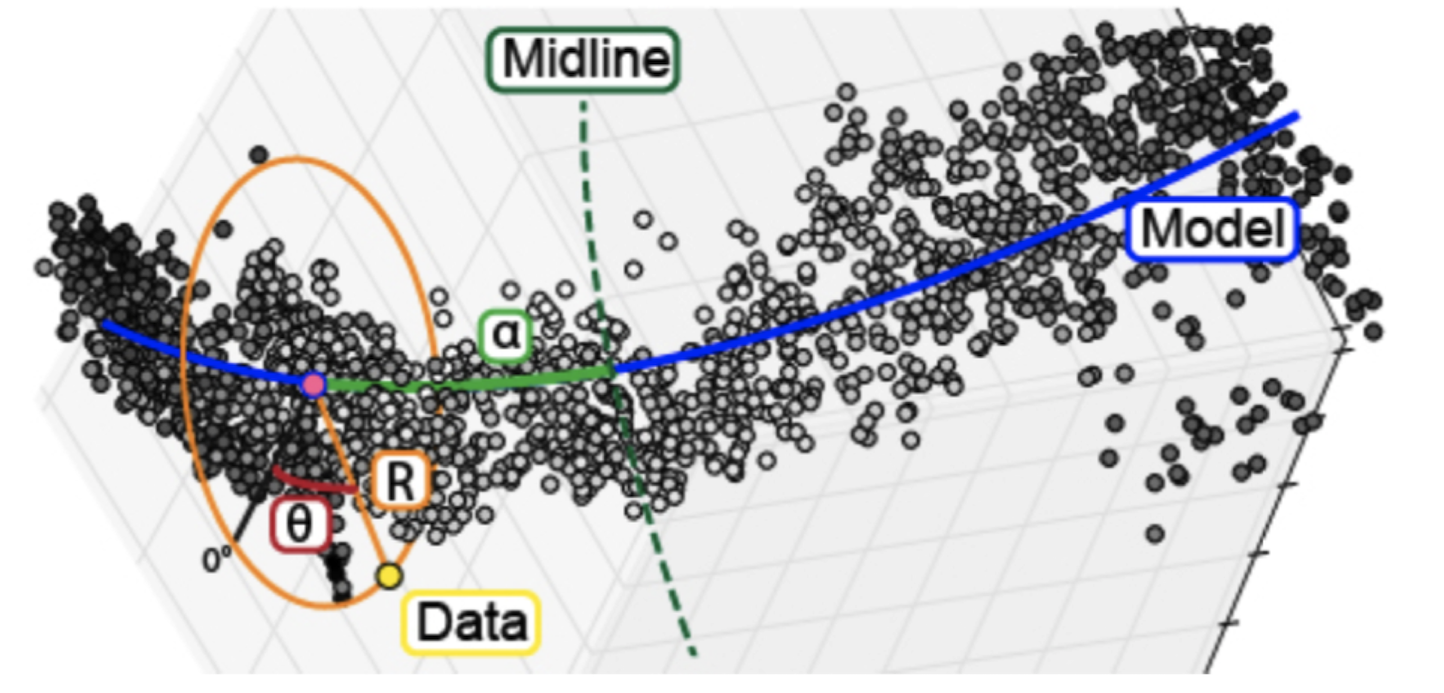
\includegraphics[width=5.55in]{figures/landmark} 

}

\caption{\label{landmark} Landmark Data of A Zebrafish Sample}\label{fig:unnamed-chunk-2}
\end{figure}

We received the raw dataset from Schwartz, a student in Professor
Barresi's Lab, who used optimization to divide the three-dimensional
shape of Zebrafish's brain into small wedges and computed the landmark,
the most representative point, of each wedge {[}1{]}. The data points
representing signals in a Zebrafish's brain is shown in \textbf{Figure
\ref{landmark}}.

\subsubsection{Programming Languages}\label{programming-languages}

Two programming languages are used in the creation of the calssification
tool: Python and \textbf{R}. Python is used to run support vector
machine models and output the results in correct format. \textbf{R} is
used generally for data cleaning and creating interactive user
interface.

\subsubsection{\texorpdfstring{Git, \texttt{knitr}, and Reproducible
Research}{Git, knitr, and Reproducible Research}}\label{git-knitr-and-reproducible-research}

Reproducible research and open source are important in this study. As
scholars place more emphasis on the reproducibility of research studies,
it is essential for us to make our code publicly available for people to
recreate both the model and the user interface.

Github and \texttt{knitr} {[}2{]} were used in this project to make the
study reproducible. Github was used to store the scripts of our final
paper and the source code of our final product which contains the final
model and the user interface. We used an \textbf{R} package called
\texttt{rticles} to write this paper. This tool allows authors to create
reproducible and dynamic technical scientific paper in \textbf{R}
Markdown. It also allows users to embed \textbf{R} code in a scientific
paper and output it into a PDF. \texttt{rticles} helps users to
efficiently put together scientific papers with similar formats {[}3{]}.

\section{Literature Review}\label{literature-review}

Research in developmental biology has relied on the analysis of
morphological phenotypes through qualitative examination of maximum
intensity projections that surrender the power of three-dimensional
data. Statistical methods to analyze three-dimensional visual data are
needed to detect subtle biological phenotypes {[}1{]}.

\subsubsection{Landmark Analysis}\label{landmark-analysis}

Landmarks describe a shape by locating a finite number of points on each
specimen. There are three basic types of landmarks: scientific,
mathematic and pseudo-landmarks. A scientific landmark is a point
assigned by an expert that corresponds between objects in some
scientifically meaningful way, for example the corner of an eye.
Mathematical landmarks are points located on an object according to some
mathematical or geometrical property of the figure. Since it does not
assume a preference of one location to another, it is particularly
useful in automated morphological recognition and analysis for
under-studied structure. Pseudo-landmarks are constructed points on an
object, located either around the outline or in between scientific or
mathematic landmarks. It is often used to approximate continuous curves
{[}4{]}. This research has chosen to calculate an automatic set of
landmarks distributed across the structure in order to avoid introducing
bias due to expectations about where biological differences should
emerge.

Schwartz et al. {[}1{]} have used the open source program, Ilastik,
which employs a training based machine learning, to eliminate the image
noise. Then they preformed principal component analysis to align
commissures between samples, reducing misalignment artifacts, and
implemented a cylindrical coordinate system which preserves image
dimensionality normally lost in maximum intensity projection (MIP),
which facilitates presentation of the data, but sacrifices much of the
complexity and relational data contained in the image. Then they reduced
the points identified by the program as belonging to the structure to a
set of landmark points that describe the shape and distribution of
signal corresponding to the structure. Finally, using the landmark
system, we are able to identify and quantify structural differences and
changes in signal distribution between wild type and mutant commissures.

\subsubsection{Support Vector Machine}\label{support-vector-machine}

Schwartz {[}1{]} used Random Forest machine leaning method to classify
the landmarks. Although the classification is quite accurate, it is
difficult to interpret the result from biological aspects. Instead of
doing classification on all of the landmarks at the same time, we
decided to do classification on one landmark at a time via Support
Vector Machine. The SVM algorithm is a classification algorithm that
provides state-of-the-art performance in a wide variety of application
domains, image classification. During the past few years, SVM has been
applied very broadly within the field of computational biology
especially in pattern recognition problems, including protein remote
homology detection, microarray gene expressions analysis, prediction of
protein-protein interactions, etc. In 1999, Jaakkola et al {[}5{]}
ushered the development of homology detection algorithms with a paper
that garnered the ``Best paper'' award at the annual Intelligent Systems
for Molecular Biology conference. Their primary insight was that
additional accuracy can be obtained by modeling the difference between
positive and negative examples. Because the homology task required
discriminating between related and unrelated sequences, explicitly
modeling the difference between these two sets of sequences yields an
extremely powerful method.

\section{Data and Variables}\label{data-and-variables}

\subsubsection{Landmark Data}\label{landmark-data}

Schwartz used optimization to divide the three-dimensional shape of
Zebrafish's brain into small wedges and computed the landmarks {[}1{]}.
The shape in \textbf{Figure \ref{landmark}} is divided into 30 circular
slices, and each slice is further divided into 8 wedges. The landmark of
each wedge is calculated by taking the median distance of all points in
each wedge, \(r\). We use the number of points in each wedge and median
\(r\) to run SVM models to run classifications.

We have 43 wild types samples (\(n_1\)) and 35 mutant samples (\(n_2\))
for training and testing. There are 152 landmarks (\(N\)) for each
sample, which resemble \textbf{Figure \ref{landmark}}, with each of them
containing the following variables:

\begin{itemize}
\tightlist
\item
  number of points in each wedge
\item
  median \(r\) (micro-meter): the median of the distances to the center
  of the slice of all the points in each wedge
\item
  \(\alpha\) (micro-meter): distance from the center of the landmark to
  the midline
\item
  \(\theta\) (radian): the degree the describes the location of a wedge
  within each slice
\end{itemize}

We used the number of points and the median \(r\) to do classification
via support vector machine. For missing median \(r\) values due to
absence of points in particular wedge, we filled them with the median
value of all the points in that wedge.

\subsubsection{Tidy Data}\label{tidy-data}

The raw landmark data is a wide table containing sample index and all
columns holding information regarding to the minimum and maximum values
of \(\alpha\) and \(\theta\), number of points, median \(r\) value, and
the true type of each sample. The value in each cell refers to either
median \(r\) value or number of points. Since all variables names in the
raw dataset, such as \texttt{-14.29\_-4.76\_-0.79\_0.0\_50\_pts} and
\texttt{-14.29\_-4.76\_-0.79\_0.0\_50\_r}, are long and hard to
interpret, we decided to restructure the raw dataset so that the new
dataset havs sample index, minimum and maximum \(\alpha\), minimum and
maximum \(\theta\), number of points, median \(r\), and type of sample
each as its own columns.

Three key functions in \texttt{tidyr} R package {[}6{]} were used:
\texttt{gather()}, \texttt{separate()}, and \texttt{spread()}.
\texttt{gather()} separated the dataset into key and value pairs for
each sample index. The key was the column name that contain essential
information that describes the position of each landmark wedge, such as
\texttt{-14.29\_-4.76\_-0.79\_0.0\_50\_r}, and the value is either the
number of points or median \(r\) value of each landmark wedge.
\texttt{separate()} divided the keys collected from \texttt{gather()},
such as \texttt{-14.29\_-4.76\_-0.79\_0.0\_50\_r}, into 5 different
columns, \texttt{min\_alpha}, \texttt{max\_alpha}, \texttt{min\_theta},
\texttt{max\_theta}, and \texttt{ptsOrR}. The \texttt{ptsOrR} variable
describes what type of information each cell contains. This was added to
the result of \texttt{gather()} that contains the sample index and
either median \(r\) or number of points of each cell. Afterwards,
\texttt{spread()} widened the already wide table by expanding the
\texttt{ptsOrR} column by creating two columns, one column representing
median \(r\) and one column representing the number of points.

\subsubsection{Dealing with Missing
Values}\label{dealing-with-missing-values}

Support Vector Machine (SVM) cannot throws away observations with
missing values. For wedges that do not have any points, median \(r\)
cannot be calculated, which means that information collected from these
wedges are eliminated when running SVMs. Wedges without points have
biologically meanings, so we should not ignore these wedges in the SVM
model. In order to get rid of the missing values, we need to
artificially pick a value to replace the missing median \(r\) values.
From a biological perspective, the reason that there is no point in a
particular wedge might be that the data points are too far away from the
scanned area to be captured. Therefore, we decided to calculate the mean
of median \(r\) of both wildetype and mutant samples, and then we
replace the missing median \(r\) values with \(2\) \(\cdot\) median
\(r\) for each landmark according to the true type of the samples to
show that the points in this wedge are too far away from the scanned
area to be captured.

\section{Support Vector Machine}\label{support-vector-machine-1}

The goal of SVM is to find a separation line
\(f(x) = (\beta_0 + \beta_1 \cdot x_1 + \beta_2 \cdot x_2)\) that
separates the data points as cleanly as possible as shown in
\textbf{Figure \ref{svmfig}} below. The optimal parameters \(\beta\) are
found by solving the optimization problem --to maximize margin subject
to certain restrictions {[}7{]}.

\begin{figure}[h]
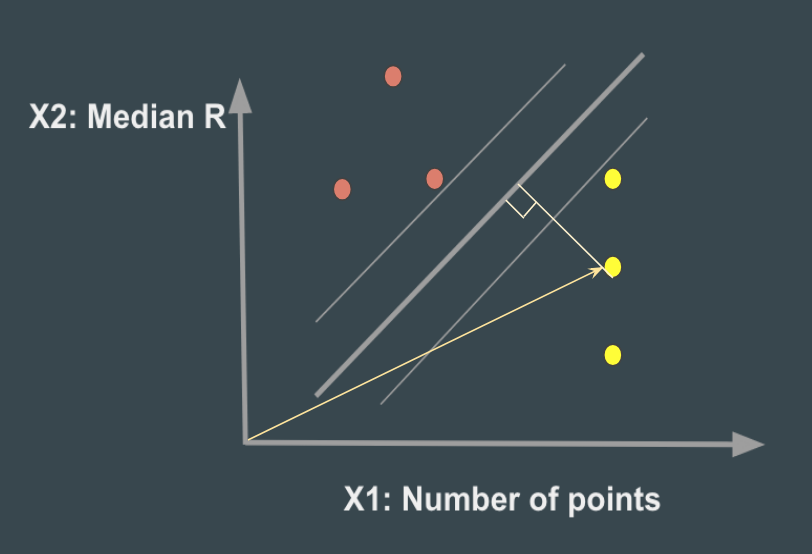
\includegraphics[width=3.12in]{figures/svm_fig} \caption{\label{svmfig} SVM model}\label{fig:unnamed-chunk-3}
\end{figure}

\begin{equation}
  \left.
  \begin{array}{l@{\,}l}
     \sum_{i=1}^n \beta_i^2 = 0 \\
     \ y_i \cdot ( \beta_0 + \beta_1 \cdot x_1 + \beta_2 \cdot x_2 ) \geq M(1-\varepsilon_i) \\
     \ \varepsilon_i \geq 0 \\
     \ \sum_{i=1}^n \varepsilon_i \leq C \\
  \end{array}
  \right.
\end{equation}

\begin{itemize}
\tightlist
\item
  \(M\): Margin is the sum of distance of the two closest points from
  each class to the separation line.
\item
  \(\varepsilon_i\) : slack variable.
\item
  \(C\): Tuning parameter, toleration of total misclassification.
\end{itemize}

The slack variable \(\varepsilon_i\) tells us where the \(i^{th}\)
observation is located, relative to the separation line and the margin.
If \(\varepsilon_i = 0\) then the \(i^{th}\) observation is on the
correct side of the margin. If \(\varepsilon_i > 0\) then the \(i^{th}\)
observation is on the wrong side of the margin. If \(\varepsilon_i > 1\)
then it is on the wrong side of the separation line.

The tuning parameter C bounds the sum of the \(\varepsilon_i\), and
therefore determines the number and severity of the violations to the
separation line and margin that we will tolerate. We can think of C as a
budget for the margin can be violated by the n observations. If
\(C = 0\) then there is no budget for violations to the margin, and it
must be the case that \(\varepsilon_1 = . . . = \varepsilon_n = 0\). For
\(C > 0\) no more than C observations can be on the wrong side of the
separation line, because if an observation is on the wrong side of the
separation line then \(\varepsilon_i > 1\). As the budget C increases,
we become more tolerant of violations to the margin, and so the margin
will widen. Conversely, as C decreases, we become less tolerant of
violations to the margin and so the margin narrows.

\(y_i\) is the vector representing the coordinate of a data point. The
dot product of \(y_i\) and the function of the separation line gives the
perpendicular distance from the data point to the separation line:

\[y_i \cdot ( \beta_0 + \beta_1 \cdot x_1 + \beta_2 \cdot x_2 )\]

If the dot product is greater than 0, the observation falls at the right
side of the separation line and vice versa.

In general, we want to find a classification that the distance from a
data point to the separation line is larger than the margin, while we
can tolerate some points being in the middle of the margins or
misclassified.

\subsubsection{Cross-Validation}\label{cross-validation}

For our project, we have access to 43 wild-type samples and 35
mutant-type samples. Due to this limited sample size, we decided to use
a leave-one-out cross validation method to test our model. For each
testing sample, we built 152 SVMs: one for each landmark. For each SVM,
we used 10-fold cross validation to select a tuning parameter C value
among 0.1, 1 and 10.

\section{Final Product: Two-Step Interactive Classification
Tool}\label{final-product-two-step-interactive-classification-tool}

We created a two-step interactive classification tool which allows users
to simply input a data file and get an visualization of the modeling
result. There are two main components in the tool:

\subsubsection{General Workflow}\label{general-workflow}

\begin{figure}[h]

{\centering 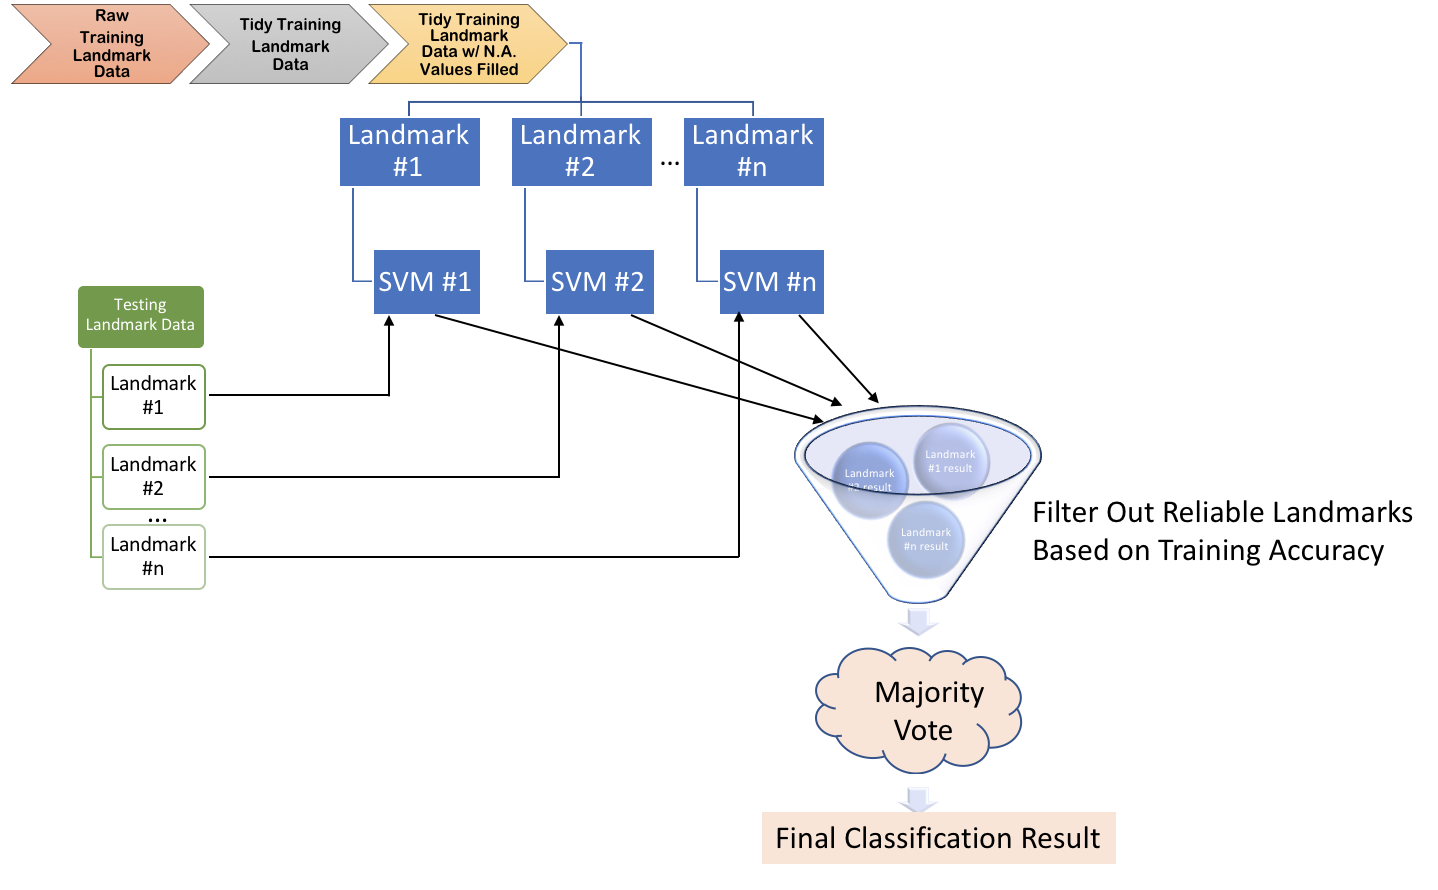
\includegraphics[width=5.55in]{figures/Figure1} 

}

\caption{\label{workflow} Summary of Workflow}\label{fig:unnamed-chunk-4}
\end{figure}

\textbf{Figure \ref{workflow}} displays the overall workflow leading to
the final product of classification. It begins with the cleaning and
restructuring of the raw landmarks data. The tidied landmarks data that
has the NA values filled contains 152 distinct landmarks. Each landmark
has its own representative SVM model that used the 77 samples out of 78
for training from applying the leave-one-out cross validation method.
That one sample that is left out from each landmark is used for testing
the model that was built from the 77 samples. Then, based on the
training accuracy of each model, only those that consist of reliable
landmarks are filtered out. The number of wild types and mutants
predicted with each model are calculated and this leads to the final
classification result of using SVMs.

\subsection{Step One: Data Processing and
Modeling}\label{step-one-data-processing-and-modeling}

This step is implemented using Python (version 3) and packages including
\texttt{pandas}, \texttt{numpy} and \texttt{sklearn}. Users would need
to run and interact with the Python script \texttt{svm.py} to preprocess
the data and build the model. Then, they would need to run another
script \texttt{analyse\_results.py} to analyse the raw results and
produce aggregated results.

The script \texttt{svm.py} contains two components: a general-purpose
\texttt{svm\_classification()} function that builds a SVM model to
classify points for a particular landmark and a \texttt{main()} function
that runs the \texttt{svm\_classification()} function for each landmark.

The script \texttt{analyse\_results.py} contains three components: a
helper function \texttt{get\_result\_file\_pathes()} that returns a list
of result file paths in the output folder; a helper function
\texttt{process\_row\_data()} that takes a path of raw data file and
returns one with accuracy scores calculated and attached; a
\texttt{main()} function that runs the two helper function to process
all raw data files and generates an aggregated \texttt{CSV} file
containing results from all samples.

\subsubsection{User Interaction}\label{user-interaction}

\begin{figure}[h]

{\centering 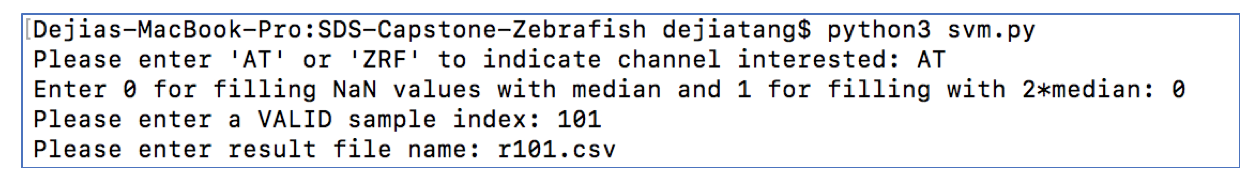
\includegraphics[width=4.49in]{figures/Figure2} 

}

\caption{\label{useri} Example of User Interaction in Step One of the User Interface}\label{fig:unnamed-chunk-5}
\end{figure}

\begin{figure}[h]
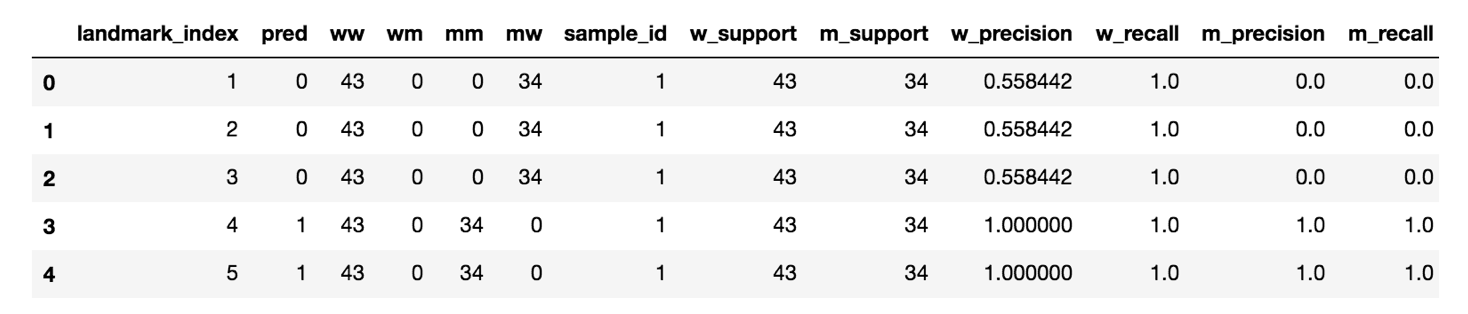
\includegraphics[width=5.03in]{figures/Figure4} \caption{\label{useri2} Example of User Interaction for Running svm.py}\label{fig:unnamed-chunk-6}
\end{figure}

As shown in \textbf{Figure \ref{useri}} and \textbf{Figure
\ref{useri2}}, several user inputs are taken from users when they run
the python scripts.

\subsubsection{Input File}\label{input-file}

Input file must contain landmark data. Variables that are needed for
classification are required to be included in the input file. In our
analysis, we used number of points in each wedge within the 3D shape and
the median \(r\) of points in each wedge.

\paragraph{Sample input file}\label{sample-input-file}

\begin{figure}[h]

{\centering 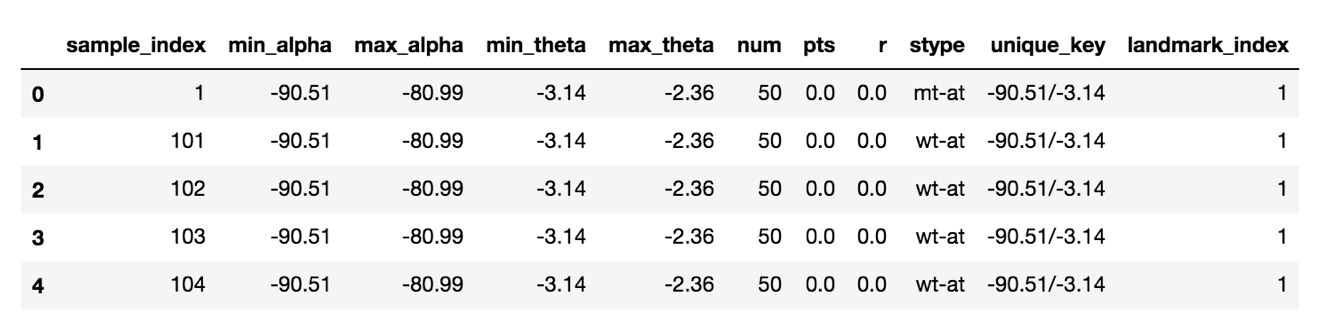
\includegraphics[width=300px]{figures/Figure3} 

}

\caption{\label{inputdata} Sample Data Input File of First Step of the User Interface}\label{fig:unnamed-chunk-7}
\end{figure}

\textbf{Figure \ref{inputdata}} shows a random sample of an input file
for the script \texttt{svm.py}. The columns \texttt{stype} (sample
type), \texttt{landmark\_index} and \texttt{sample\_index} are required
and the other two columns (\texttt{pts} and \texttt{r} in this example)
are the two parameters used for building SVM.

\subsubsection{Output File}\label{output-file}

\begin{figure}[h]

{\centering 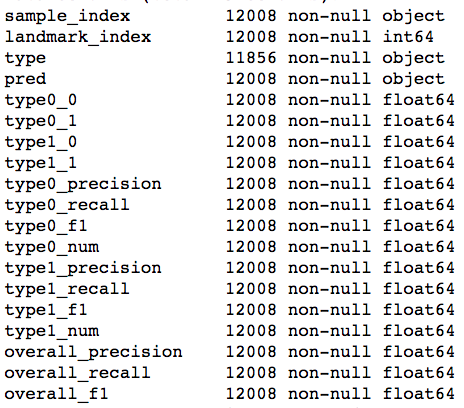
\includegraphics[width=300px]{figures/Figure5} 

}

\caption{\label{outputdata} Sample Data Output File of First Step of the User Interface}\label{fig:unnamed-chunk-8}
\end{figure}

\textbf{Figure \ref{outputdata}} shows the columns of the final result
file produced by the \texttt{analyse\_results.py} script. The first four
columns describe the testing sample's information while the rest of the
columns are all precision statistics describing the accuracy of the
built model. The descriptions of all of the columns are displayed as
follows:

\begin{itemize}
\tightlist
\item
  \texttt{sample\_index}: sample index of the testing sample
\item
  \texttt{landmark\_index}: the index of the landmark
\item
  \texttt{type}: the actual type of the testing sample
\item
  \texttt{pred}: the prediction made by the model
\item
  \texttt{type0\_0}: number of type 0 samples that are classified as
  type 0 in the corresponding landmark's SVM
\item
  \texttt{type0\_1}: number of type 0 samples that are classified as
  type 1 in the corresponding landmark's SVM
\item
  \texttt{type1\_1}: number of type 1 samples that are classified as
  type 1 in the corresponding landmark's SVM
\item
  \texttt{type1\_0}: number of type 1 samples that are classified as
  type 0 in the corresponding landmark's SVM
\item
  \texttt{type0\_precision}: percentage of samples that are classified
  by the corresponding landmark's SVM as type 0 are really of type 0
\item
  \texttt{type0\_recall}: percentage of type 0 samples that are
  classified by the corresponding landmark's SVM as type 0.
\item
  \texttt{type0\_f1}: harmonic mean of \texttt{type0\_precision} and
  \texttt{type0\_recall}
\item
  \texttt{type0\_num}: number of type 0 samples in the training dataset
\item
  \texttt{type1\_precision}: percentage of samples that are classified
  by the corresponding landmark's SVM as type 1 are really of type 1
\item
  \texttt{type1\_recall}: percentage of type 1 samples that are
  classified by the corresponding landmark's SVM as type 1
\item
  \texttt{type1\_f1}: harmonic mean of \texttt{type1\_precision} and
  \texttt{type1\_recall}
\item
  \texttt{type1\_num}: number of type 1 samples in the training dataset
\item
  \texttt{overall\_precision}: weighted average of
  \texttt{type0\_precision} and \texttt{type1\_precision}
\item
  \texttt{overall\_recall}: weighted average of \texttt{type0\_recall}
  and \texttt{type1\_recall}
\item
  \texttt{overall\_f1}: weighted average of \texttt{type0\_f1} and
  \texttt{type1\_f1}
\end{itemize}

\subsection{Step Two: Interactive Visualization
Tool}\label{step-two-interactive-visualization-tool}

After building SVM models in step one, we insert the output from the SVM
models into step two to visualize the results. Steps two uses the
accuracy scores output from step one to create a user-friendly app which
generates visualizations to help users to understand the SVM results.

The repository containing the shiny app can be accessed by doing the
following:

\begin{Shaded}
\begin{Highlighting}[]
\KeywordTok{install.packages}\NormalTok{(}\StringTok{"devtools"}\NormalTok{)}
\NormalTok{devtools}\OperatorTok{::}\KeywordTok{install_github}\NormalTok{(}\StringTok{"liwencong1995/SDS-Capstone-Zebrafish"}\NormalTok{)}
\end{Highlighting}
\end{Shaded}

The file containing the source code of the shiny app can be found in
\texttt{9.FinalModel} folder of the repository. The file is named as
\texttt{shiny\_app.R}.

\subsubsection{Input 1: Data File and
Variables}\label{input-1-data-file-and-variables}

Input \texttt{CSV} data file must be stored in a folder called
\texttt{data} under your working directory, and the \texttt{CSV} file
must be named as \texttt{output\_data.csv}. If you do not know what your
working directory is, you can check it by using the function
\texttt{getwd()} in base \textbf{R}.

All SVM models from step one produce the following 9 accuracy
measurements:

\begin{enumerate}
\def\labelenumi{\arabic{enumi}.}
\tightlist
\item
  Precision score of type 0
\item
  Recall score of type 0
\item
  F1 score of type 0
\item
  Precision score of type 1
\item
  Recall score of type 1
\item
  F1 score of type 1
\item
  Overall precision score
\item
  Overall recall score
\item
  Overall F1 score
\end{enumerate}

These 9 accuracy scores are the variables needed in the second step of
the user interface to create the visualizations.

\subsubsection{Input 2: User Inputs}\label{input-2-user-inputs}

Users can select \texttt{channel} and \texttt{sample\ index} to filter
the input dataset to only keep the observations that users are
interested in.

In addition, users can set the threshold of the following variables:

\begin{itemize}
\tightlist
\item
  Overall precision score
\item
  Overall recall score
\item
  Overall F1 score
\end{itemize}

The dataset used to create the visualizations is rendered every time
users change one or multiple thresholds. Our app filters out the
observations that do not fulfill the threshold requirements and uses the
remaining dataset to update the histograms and heat maps.

\subsubsection{Output: Interactive User
Interface}\label{output-interactive-user-interface}

This interactive user interface was built upon several \textbf{R}
packages:

\begin{itemize}
\tightlist
\item
  \texttt{dplyr} {[}8{]}
\item
  \texttt{data.table} {[}9{]}
\item
  \texttt{ggplot2} {[}10{]}
\item
  \texttt{shiny} {[}11{]}
\end{itemize}

We visualize the 9 accuracy scores by using both histograms and the
corresponding heat maps that display the scores included in the
histograms in rectangular shapes that are colored with different shades
of blue according to their magnitudes. The positions of the shapes are
determined with respect to their relative positions within the
biological structure. In the study of Zebrafish, we used the relative
positions of the wedges used in landmark analysis to determine the
position of the wedges in the heat map.

There are 10 tabs included in the user interface of the app: 1 Accuracy
Threshold Summary tab and 9 accuracy score visualization tabs.

\begin{figure}[h]

{\centering 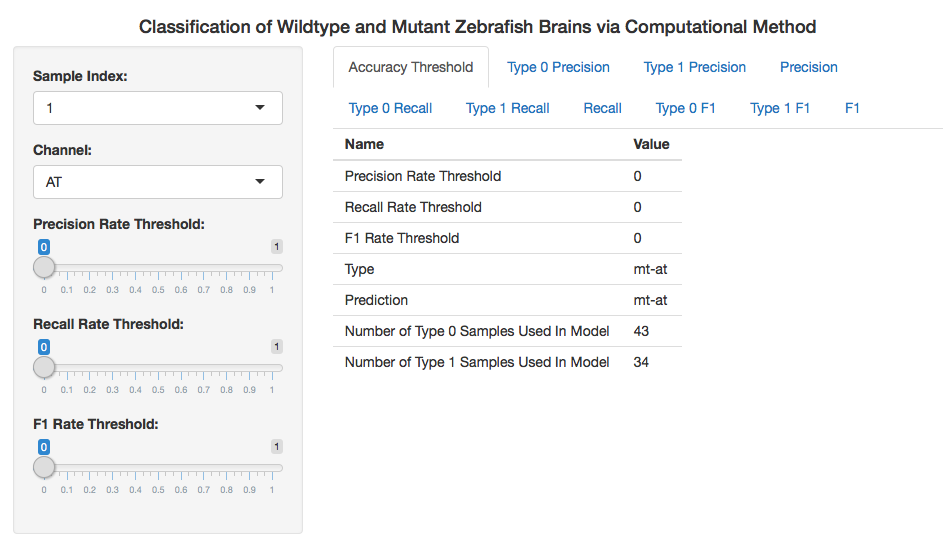
\includegraphics[width=3.66in]{figures/shiny1} 

}

\caption{\label{shiny1} User Interface: Accuracy Threshold Summary Tab of AT Channel}\label{fig:unnamed-chunk-10}
\end{figure}

\textbf{Figure \ref{shiny1}} displays the Accuracy Score Threshold
Summary tab of the first sample of AT channel. Users can drag the dot on
the slidebar to set the thresholds of overall precision, recall, and f1
scores. The threshold of the three scores are updated in the summary
table. Default thresholds are 0 for all three accuracy measurements. We
then use the landmark observations that fulfill the threshold
requirements to predict the type of the sample of choice by doing a
majority vote. We simply count the total number of landmarks that are
classified as type 0 and type 1, and then we determine whether there are
more of them that are classified as type 0 or type 1. The type that gets
more vote is the predicted type of the sample. The resulting predicted
sample type is also updated in the summary table.

Other information, such as the true type of the sample and the number of
wild types and mutants used in training the SVM models are also included
in the summary table.

\begin{figure}[h]

{\centering 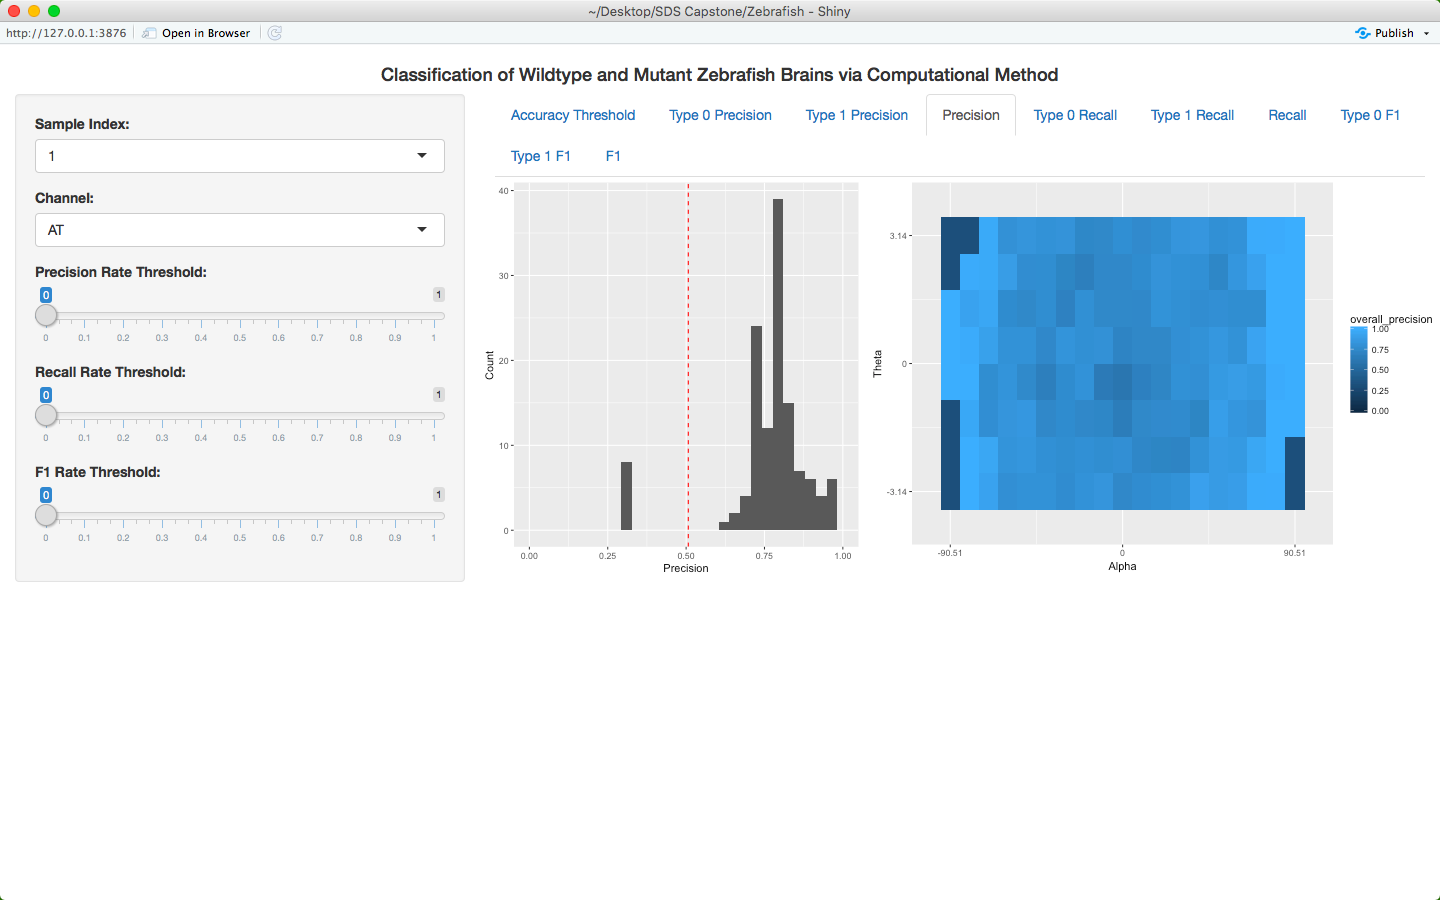
\includegraphics[width=4.92in]{figures/shiny2} 

}

\caption{\label{shiny2} User Interface: Precision Score Visualization Tab of AT Channel}\label{fig:unnamed-chunk-11}
\end{figure}

\textbf{Figure \ref{shiny2}} displays the Precision Score Visualization
tab of the first sample of AT channel. In this case, all three
thresholds are at default level, 0. All landmarks' precision scores are
shown in both the histogram and the heat map.

\begin{figure}[h]

{\centering 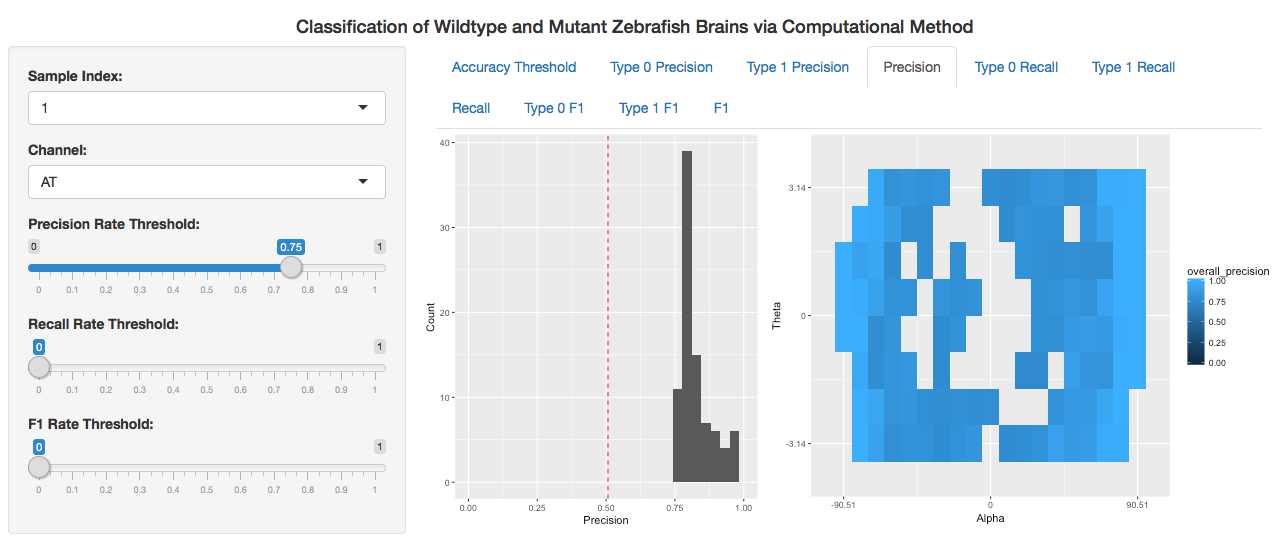
\includegraphics[width=4.9in]{figures/shiny3} 

}

\caption{\label{shiny3} User Interface: Precision Score Visualization Tab of AT Channel, with precision threshold = 0.75}\label{fig:unnamed-chunk-12}
\end{figure}

\textbf{Figure \ref{shiny3}} also displays the Precision Score
Visualization tab of the first sample of AT channel. In this case,
recall and f1 scores' thresholds are at default level and precision
threshold is set to be 0.75. Therefore, only landmarks that have
precision scores that are equal to or greater than 0.75 are shown in the
visualizations. As shown in the histogram, all values less than 0.75 are
removed from the histogram in figure 6. Some of the blocks in figure 6
are turned into blank blocks after the precision threshold is increased
to 0.75.

\begin{figure}[h]

{\centering 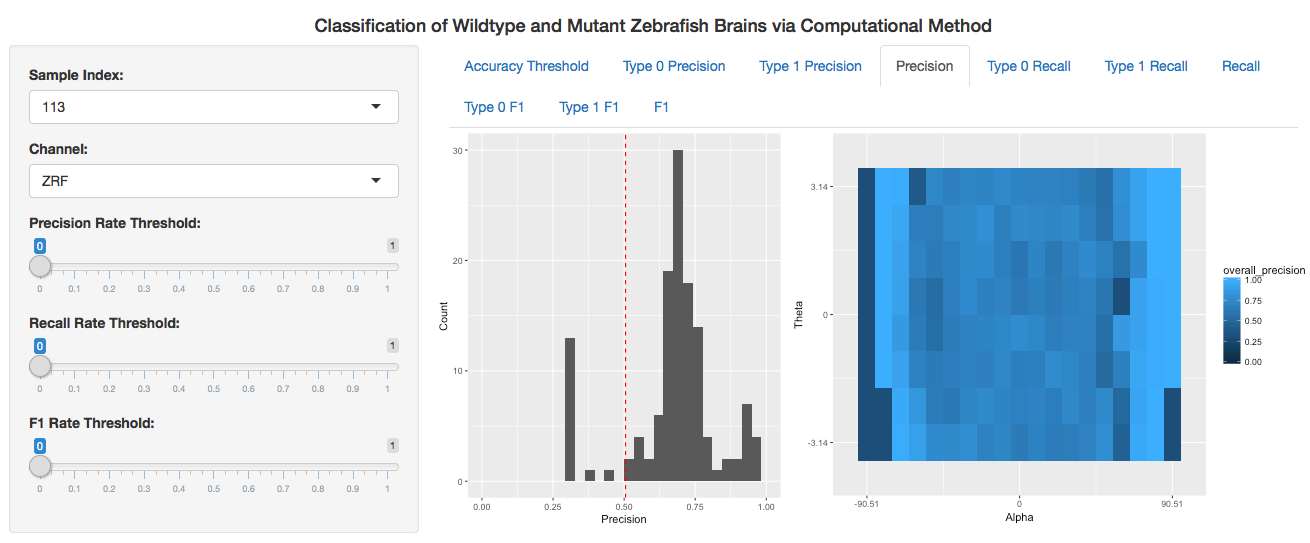
\includegraphics[width=5.04in]{figures/shiny8} 

}

\caption{\label{shiny4} User Interface: F1 Score Visualization Tab of ZRF Channel}\label{fig:unnamed-chunk-13}
\end{figure}

Users can also choose to observe the SVM results of ZRF channel.
\textbf{Figure \ref{shiny4}} displays the Precision Score Visualization
tab of the first sample of ZRF channel with all thresholds equal to 0.
More sample visualizations of other accuracy scores can be found in
Appendix A.

\section{Conclusion and Discussion}\label{conclusion-and-discussion}

\subsection{Strengths}\label{strengths}

Our final product has several strengths:

\subsubsection{Easy Interpretation}\label{easy-interpretation}

In the previously used random forest method, the number of predictors
\(p\) exceeds the number of samples. Schwartz {[}1{]} applied the
Principle Component Analysis to reduce the dimension of the predictors.
The problem with reducing the dimension is that the parameters gaining
weights at last are linear combinations of the original landmarks. While
the patterns of the first several projections still make sense, the
minor projections are very random and thus difficult to interpret.

The SVM model run on each landmark data gives insightful analysis of
which landmark, or which part of the Zebrafish brain, has more power in
making predictions.

\subsubsection{Implementing User
Feedback}\label{implementing-user-feedback}

We have implemented feedback from users in our user interface.
Originally, our shiny app only produced visualizations of one channel's
data, but we added an additional variable, \texttt{channel}, for users
to analyze three-dimensional data with more or multiple channels.
Because of this improvement, it is more convenient for users to compare
and contrast results from different channels.

\subsection{Limitations and
Improvements}\label{limitations-and-improvements}

\subsubsection{Interaction Between Channels and
sections}\label{interaction-between-channels-and-sections}

Our SVM model only make prediction based on a single channel's
information and the SVM is run for one single landmark at a time. It
does not consider the interactions between channels and between
different sections of the sample.

\subsubsection{Iterating Machine
Learning}\label{iterating-machine-learning}

Instead of cross-validation, iterating machine learning method could
achieve better results. In iterative machine learning, we repeat the
process of training and testing several times. In the first round, the
user gives examples of objects belonging to specific classes and the
machine learning algorithm is trained with this data. In the second
round, the algorithm shows examples of objects it thinks that belong to
these classes. Now, the user merely adds objects to the improved
training set which the machine learning algorithm has put into a wrong
class. That is, the user only corrects the ``misunderstandings'' of the
algorithm. In this way, we can concentrate on difficult examples of
objects that are hard to classify. Such objects may lie close to the
decision boundaries or in the periphery in the multidimensional feature
space. This iterative process is continued until the machine learning
algorithm does not make any mistakes or the classification results do
not improve anymore. It will improve our classification results and thus
is likely to help make better predictions for unknown type {[}12{]}.

\subsection{Future Study}\label{future-study}

\subsubsection{Interaction Between
Channels}\label{interaction-between-channels}

If more time is given, we could add factors that describe the
interaction between channels into our SVM model in order to combine
information from multiple channels to predict sample type.

\subsubsection{Improving User Interface}\label{improving-user-interface}

Since we have only received feedback from three users at Smith College,
we would love to receive more feedback from other scientists and improve
our model and user interface accordingly.

\subsubsection{Improving Model Accuracy}\label{improving-model-accuracy}

\section{Acknowledgements}\label{acknowledgements}

This project was completed in partial fulfillment of the requirements of
SDS 410: SDS Capstone. This course is offered by the Statistical and
Data Sciences Program at Smith College, and was taught by Professor
Benjamin Baumer in Spring 2018.

\newpage

\section{Appendix A: Shiny App Accuracy Score
Visualizations}\label{appendix-a-shiny-app-accuracy-score-visualizations}

\subsection{Recall Score Visualization tab of the first sample of AT
channel}\label{recall-score-visualization-tab-of-the-first-sample-of-at-channel}

\begin{figure}[h]

{\centering 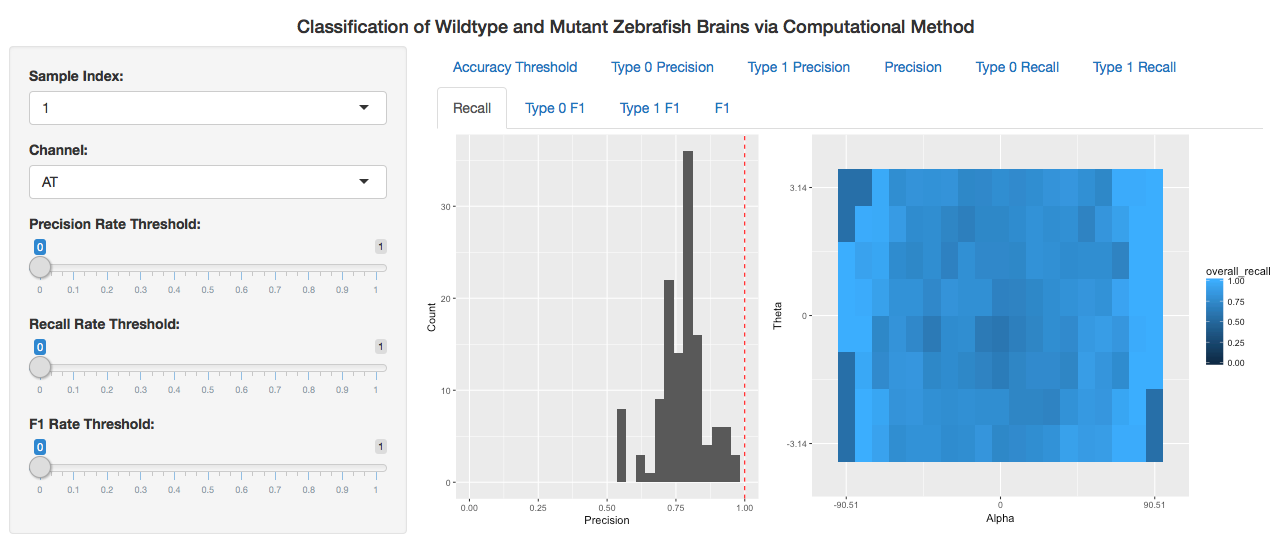
\includegraphics[width=4.91in]{figures/shiny4} 

}

\caption{User Interface: Recall Score Visualization Tab of AT Channel}\label{fig:shiny4}
\end{figure}

\subsection{Recall Score Visualization tab of the first sample of AT
channel with recall threshold equals to
0.75}\label{recall-score-visualization-tab-of-the-first-sample-of-at-channel-with-recall-threshold-equals-to-0.75}

\begin{figure}[h]

{\centering 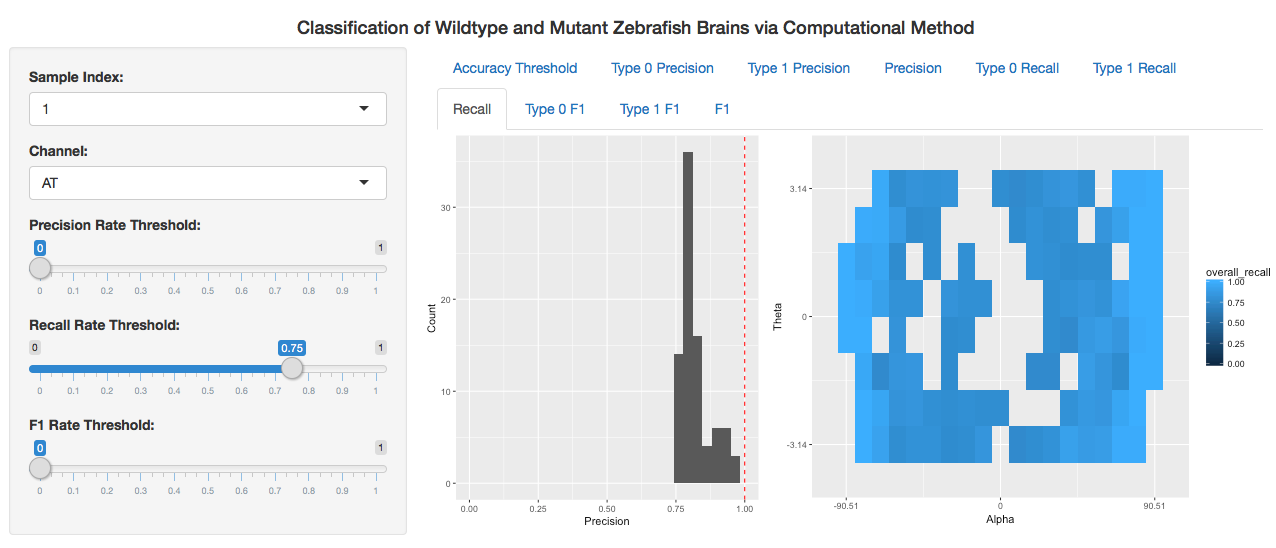
\includegraphics[width=4.91in]{figures/shiny5} 

}

\caption{User Interface: Recall Score Visualization Tab of AT Channel, with recall threshold = 0.75}\label{fig:shiny5}
\end{figure}

\newpage

\subsection{F1 Score Visualization tab of the first sample of AT
channel}\label{f1-score-visualization-tab-of-the-first-sample-of-at-channel}

\begin{figure}[h]

{\centering 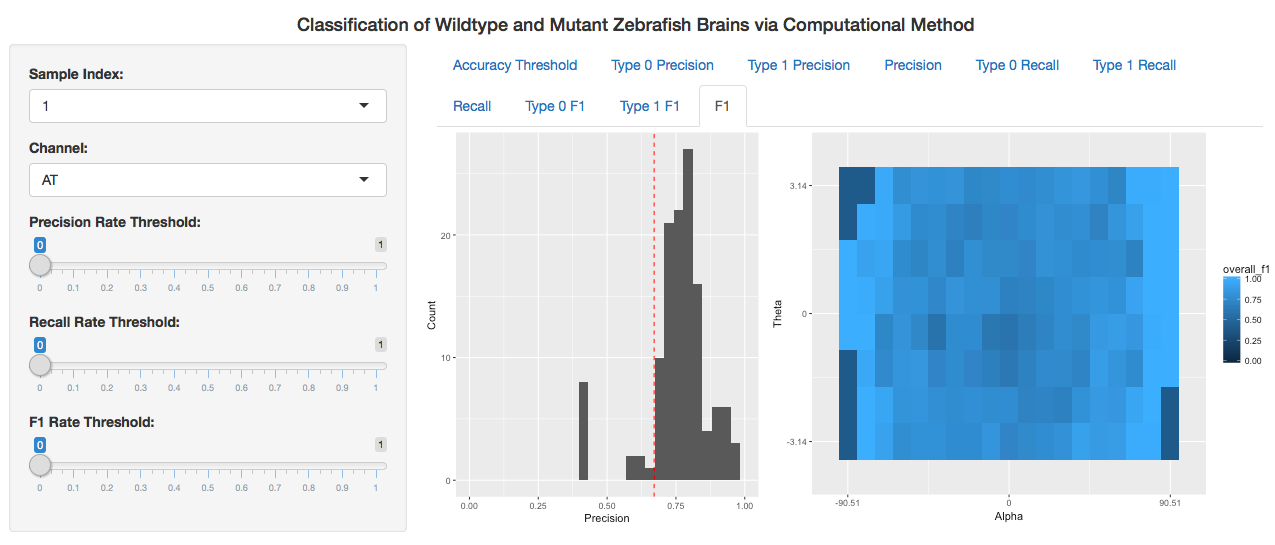
\includegraphics[width=4.9in]{figures/shiny6} 

}

\caption{User Interface: F1 Score Visualization Tab of AT Channel}\label{fig:shiny6}
\end{figure}

\subsection{F1 Score Visualization tab of the first sample of AT channel
with f1 threshold equals to
0.75}\label{f1-score-visualization-tab-of-the-first-sample-of-at-channel-with-f1-threshold-equals-to-0.75}

\begin{figure}[h]

{\centering 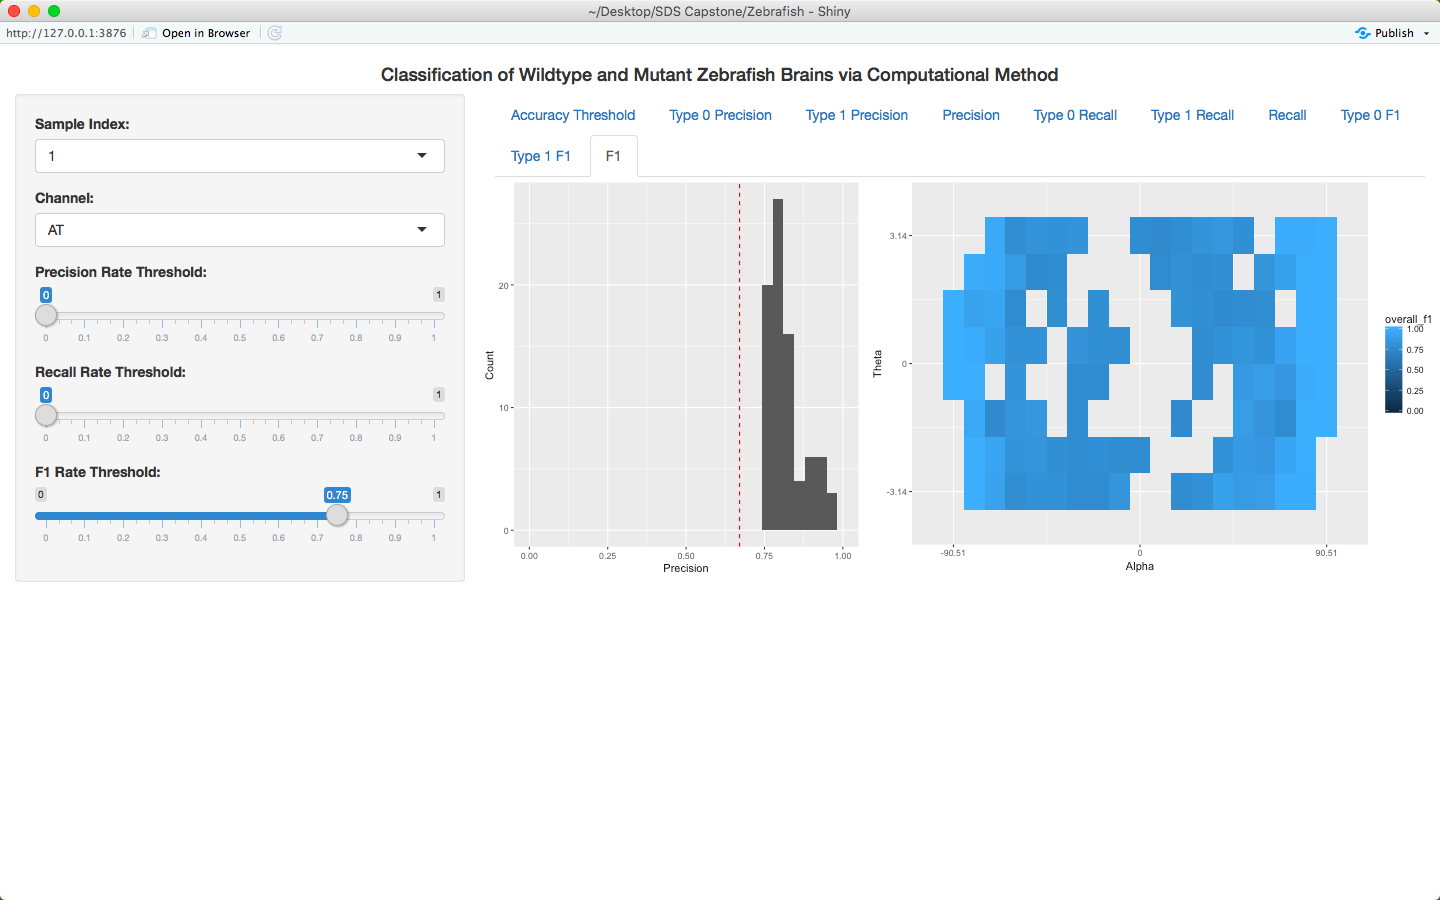
\includegraphics[width=4.9in]{figures/shiny7} 

}

\caption{User Interface: F1 Score Visualization Tab of AT Channel, with f1 threshold = 0.75}\label{fig:shiny7}
\end{figure}

\newpage

\section{Appendix B: Source Code for User
Interface}\label{appendix-b-source-code-for-user-interface}

\subsection{Support Vector Machine}\label{support-vector-machine-2}

\begin{Shaded}
\begin{Highlighting}[]
\NormalTok{import pandas as pd}
\NormalTok{import numpy as np}
\NormalTok{from sklearn.metrics import confusion_matrix, classification_report}
\NormalTok{from sklearn.model_selection import GridSearchCV}
\NormalTok{from sklearn.svm import SVC}
\NormalTok{from sklearn.metrics import f1_score, precision_score, recall_score}

\StringTok{'''}
\StringTok{A function that builds a SVM model with linear kernel to classify points}
\StringTok{to two classes.}

\StringTok{Inputs:}
\StringTok{training_landmarks - a pandas dataframe containing all training landmark}
\StringTok{                     data.}
\StringTok{index              - a perticular landmark id of interest. eg. '}\DecValTok{101}\StringTok{'}
\StringTok{x_names            - a list of explanatory variable names.}
\StringTok{                     eg. ['}\NormalTok{pts}\StringTok{', '}\NormalTok{r}\StringTok{']}
\StringTok{y_name             - a string representing response variable name.}
\StringTok{                     eg. '}\NormalTok{stype}\StringTok{'}
\StringTok{class0             - name of the first class. eg. '}\NormalTok{wt}\OperatorTok{-}\NormalTok{at}\StringTok{'}
\StringTok{class1             - name of the second class. eg. '}\NormalTok{mt}\OperatorTok{-}\NormalTok{at}\StringTok{'}
\StringTok{C_values           - a list of tunning variable C (penalty parameter}
\StringTok{                     of the error term) that the method would grid-search}
\StringTok{                     on. Default value is [0.1, 1, 10].}

\StringTok{Output:}
\StringTok{svm                - the SVM model trained from the training dataset}
\StringTok{type0_0            - among the training samples, the number of class0}
\StringTok{                     samples with chosen landmark predicted as class0}
\StringTok{type0_1            - among the training samples, the number of class0}
\StringTok{                     samples with chosen landmark predicted as class1}
\StringTok{type1_1            - among the training samples, the number of class1}
\StringTok{                     samples with chosen landmark predicted as class1}
\StringTok{type1_0            - among the training samples, the number of class1}
\StringTok{                     samples with chosen landmark predicted as class0}
\StringTok{'''}
\NormalTok{def }\KeywordTok{svm_classification}\NormalTok{(training_landmarks, index, x_names, y_name, class0,}
\NormalTok{        class1, }\DataTypeTok{C_values =}\NormalTok{ [}\FloatTok{0.1}\NormalTok{, }\DecValTok{1}\NormalTok{, }\DecValTok{10}\NormalTok{] )}\OperatorTok{:}
\StringTok{    }\CommentTok{# filter out the landmarks needed}
\StringTok{    }\NormalTok{chosenLandmark =}\StringTok{ }\NormalTok{landmarks[landmarks.landmark_index}\OperatorTok{==}\NormalTok{index]}
\NormalTok{    chosenLandmark =}\StringTok{ }\NormalTok{chosenLandmark[}\KeywordTok{np.isfinite}\NormalTok{(chosenLandmark[}\StringTok{'r'}\NormalTok{])]}
    
    \CommentTok{# create training and testing data}
\NormalTok{    X =}\StringTok{ }\NormalTok{chosenLandmark[x_names]}
\NormalTok{    y =}\StringTok{ }\NormalTok{chosenLandmark[y_name]}

    \CommentTok{# check whether both classes exist}
\NormalTok{    count_}\DecValTok{1}\NormalTok{ =}\StringTok{ }\NormalTok{chosenLandmark[y_name]}\KeywordTok{.str.contains}\NormalTok{(class1)}\KeywordTok{.sum}\NormalTok{()}
\NormalTok{    count_}\DecValTok{0}\NormalTok{ =}\StringTok{ }\NormalTok{chosenLandmark[y_name]}\KeywordTok{.str.contains}\NormalTok{(class0)}\KeywordTok{.sum}\NormalTok{()}

    \ControlFlowTok{if}\NormalTok{ (count_}\DecValTok{1} \OperatorTok{<}\StringTok{ }\DecValTok{2}\NormalTok{ or count_}\DecValTok{0} \OperatorTok{<}\StringTok{ }\DecValTok{2}\NormalTok{)}\OperatorTok{:}
\StringTok{        }\NormalTok{return None, None, None, None, None}

    \CommentTok{# find the best C value by cross-validation}
\NormalTok{    tuned_parameters =}\StringTok{ }\NormalTok{[\{}\StringTok{'C'}\OperatorTok{:}\StringTok{ }\NormalTok{C_values\}]}
\NormalTok{    clf =}\StringTok{ }\KeywordTok{GridSearchCV}\NormalTok{(}
        \KeywordTok{SVC}\NormalTok{(}\DataTypeTok{kernel=}\StringTok{'linear'}\NormalTok{),}
\NormalTok{        tuned_parameters, }\DataTypeTok{cv=}\DecValTok{10}\NormalTok{, }\DataTypeTok{scoring=}\StringTok{'accuracy'}\NormalTok{)}
    \KeywordTok{clf.fit}\NormalTok{(X.values, y.values)}
\NormalTok{    best_c =}\StringTok{ }\NormalTok{clf.best_params_[}\StringTok{'C'}\NormalTok{]}
    
\NormalTok{    svc =}\StringTok{ }\KeywordTok{SVC}\NormalTok{(}\DataTypeTok{C=}\NormalTok{best_c, }\DataTypeTok{kernel=}\StringTok{'linear'}\NormalTok{)}
    \KeywordTok{svc.fit}\NormalTok{(X, y)}
    
\NormalTok{    prediction =}\StringTok{ }\KeywordTok{svc.predict}\NormalTok{(X)}

    \CommentTok{# print confusion matrix}
    \KeywordTok{print}\NormalTok{(}\StringTok{"confusion matrix: "}\NormalTok{)}
\NormalTok{    cm =}\StringTok{ }\KeywordTok{confusion_matrix}\NormalTok{(y, prediction)}
\NormalTok{    cm_df =}\StringTok{ }\KeywordTok{pd.DataFrame}\NormalTok{(cm.T, }\DataTypeTok{index=}\NormalTok{svc.classes_, }\DataTypeTok{columns=}\NormalTok{svc.classes_)}
    \KeywordTok{print}\NormalTok{(cm_df)}

    \CommentTok{# Statistics of training precision:}
    \CommentTok{# number of wild type samples with this landmark}
    \CommentTok{# predicted as wild type.}
\NormalTok{    type0_}\DecValTok{0}\NormalTok{ =}\DecValTok{0}
    \CommentTok{# number of wild type samples with this landmark}
    \CommentTok{# predicted as mutant type.}
\NormalTok{    type0_}\DecValTok{1}\NormalTok{ =}\StringTok{ }\DecValTok{0}
    \CommentTok{# number of mutant type samples with this landmark}
    \CommentTok{# predicted as mutant type.}
\NormalTok{    type1_}\DecValTok{1}\NormalTok{ =}\StringTok{ }\DecValTok{0}
    \CommentTok{# number of mutant type samples with this landmark}
    \CommentTok{# predicted as wild type.}
\NormalTok{    type1_}\DecValTok{0}\NormalTok{ =}\StringTok{ }\DecValTok{0}
    
    \ControlFlowTok{for}\NormalTok{ i }\ControlFlowTok{in} \KeywordTok{range}\NormalTok{ (}\KeywordTok{len}\NormalTok{(y))}\OperatorTok{:}
\StringTok{        }\NormalTok{_y =}\StringTok{ }\NormalTok{y.values[i]}
\NormalTok{        _p =}\StringTok{ }\NormalTok{prediction[i]}

        \ControlFlowTok{if}\NormalTok{ _y}\OperatorTok{==}\NormalTok{class1 and _p}\OperatorTok{==}\NormalTok{class1}\OperatorTok{:}
\StringTok{            }\NormalTok{type1_}\DecValTok{1}\NormalTok{ =}\StringTok{ }\NormalTok{type1_}\DecValTok{1} \OperatorTok{+}\StringTok{ }\DecValTok{1}
\NormalTok{        elif _y}\OperatorTok{==}\NormalTok{class1 and _p}\OperatorTok{==}\NormalTok{class0}\OperatorTok{:}
\StringTok{            }\NormalTok{type1_}\DecValTok{0}\NormalTok{ =}\StringTok{ }\NormalTok{type1_}\DecValTok{0} \OperatorTok{+}\StringTok{ }\DecValTok{1}
\NormalTok{        elif _y}\OperatorTok{==}\NormalTok{class0 and _p}\OperatorTok{==}\NormalTok{class0}\OperatorTok{:}
\StringTok{            }\NormalTok{type0_}\DecValTok{0}\NormalTok{ =}\StringTok{ }\NormalTok{type0_}\DecValTok{0} \OperatorTok{+}\StringTok{ }\DecValTok{1}
\NormalTok{        elif _y}\OperatorTok{==}\NormalTok{class0 and _p}\OperatorTok{==}\NormalTok{class1}\OperatorTok{:}
\StringTok{            }\NormalTok{type0_}\DecValTok{1}\NormalTok{ =}\StringTok{ }\NormalTok{type0_}\DecValTok{1} \OperatorTok{+}\StringTok{ }\DecValTok{1}
    
\NormalTok{    return svc, type0_}\DecValTok{0}\NormalTok{, type0_}\DecValTok{1}\NormalTok{, type1_}\DecValTok{1}\NormalTok{, type1_}\DecValTok{0}


\ControlFlowTok{if}\NormalTok{ __name__ }\OperatorTok{==}\StringTok{ "__main__"}\OperatorTok{:}
\StringTok{    }\CommentTok{# Get Datafile}
\StringTok{    }\NormalTok{landmarks =}\StringTok{ }\KeywordTok{pd.DataFrame}\NormalTok{()}
    \ControlFlowTok{while}\NormalTok{(landmarks.shape[}\DecValTok{0}\NormalTok{]}\OperatorTok{<}\DecValTok{2}\NormalTok{)}\OperatorTok{:}
\StringTok{        }\NormalTok{filename =}\StringTok{ }\KeywordTok{str}\NormalTok{(}\KeywordTok{input}\NormalTok{(}\StringTok{"Please enter dataset's path: "}\NormalTok{))}
\NormalTok{        try}\OperatorTok{:}
\StringTok{            }\NormalTok{landmarks =}\StringTok{ }\KeywordTok{pd.read_csv}\NormalTok{(filename)}
\NormalTok{        except Exception}\OperatorTok{:}
\StringTok{            }\KeywordTok{print}\NormalTok{ (}\StringTok{"Error in reading the file.}
\StringTok{                Please check whether file exists."}\NormalTok{)}

    \CommentTok{# Column names}
\NormalTok{    columns =}\StringTok{ }\KeywordTok{list}\NormalTok{(landmarks)}
    \CommentTok{# Check column names}
    \ControlFlowTok{if} \StringTok{'stype'}\NormalTok{ not }\ControlFlowTok{in}\NormalTok{ columns}\OperatorTok{:}
\StringTok{        }\KeywordTok{print}\NormalTok{(}\StringTok{"Incorrect column names: Please}
\StringTok{            name your sample type's column as 'stype' "}\NormalTok{)}
        \KeywordTok{exit}\NormalTok{()}
    \ControlFlowTok{if} \StringTok{'sample_index'}\NormalTok{ not }\ControlFlowTok{in}\NormalTok{ columns}\OperatorTok{:}
\StringTok{        }\KeywordTok{print}\NormalTok{(}\StringTok{"Incorrect column names: Please name your}
\StringTok{            sample index's column as 'sample_index' "}\NormalTok{)}
        \KeywordTok{exit}\NormalTok{()}
    \ControlFlowTok{if} \StringTok{'landmark_index'}\NormalTok{ not }\ControlFlowTok{in}\NormalTok{ columns}\OperatorTok{:}
\StringTok{        }\KeywordTok{print}\NormalTok{(}\StringTok{"Incorrect column names: Please name your}
\StringTok{            landmark index's column as 'landmark_index' "}\NormalTok{)}
        \KeywordTok{exit}\NormalTok{()}

    \CommentTok{# Get Parameters' column names}
\NormalTok{    parameters =}\StringTok{ }\KeywordTok{list}\NormalTok{(}\KeywordTok{set}\NormalTok{(columns) }\OperatorTok{-}
\StringTok{        }\KeywordTok{set}\NormalTok{([}\StringTok{'stype'}\NormalTok{, }\StringTok{'sample_index'}\NormalTok{, }\StringTok{'landmark_index'}\NormalTok{]))}

    \CommentTok{# Get class names}
\NormalTok{    class0 =}\StringTok{ ''}
\NormalTok{    class1 =}\StringTok{ ''}
\NormalTok{    classes =}\StringTok{ }\KeywordTok{list}\NormalTok{(}\KeywordTok{set}\NormalTok{(landmarks[}\StringTok{'stype'}\NormalTok{].values))}
    \ControlFlowTok{while}\NormalTok{ (class0 not }\ControlFlowTok{in}\NormalTok{ classes)}\OperatorTok{:}
\StringTok{        }\NormalTok{class0 =}\StringTok{ }\KeywordTok{str}\NormalTok{(}\KeywordTok{input}\NormalTok{(}\StringTok{"Please enter name of type 0: "}\NormalTok{))}
    \ControlFlowTok{while}\NormalTok{ (class1 not }\ControlFlowTok{in}\NormalTok{ classes)}\OperatorTok{:}
\StringTok{        }\NormalTok{class1 =}\StringTok{ }\KeywordTok{str}\NormalTok{(}\KeywordTok{input}\NormalTok{(}\StringTok{"Please enter name of type 1: "}\NormalTok{))}

    \CommentTok{# Remove rows with NaN values}
    \ControlFlowTok{for}\NormalTok{ parameter }\ControlFlowTok{in}\NormalTok{ parameters}\OperatorTok{:}
\StringTok{        }\NormalTok{landmarks =}\StringTok{ }\NormalTok{landmarks[}\KeywordTok{np.isfinite}\NormalTok{(landmarks[parameter])]}

    \CommentTok{# Get sample id}
\NormalTok{    sample =}\StringTok{ }\KeywordTok{pd.DataFrame}\NormalTok{()}
    \ControlFlowTok{while}\NormalTok{(sample.shape[}\DecValTok{0}\NormalTok{]}\OperatorTok{<}\DecValTok{2}\NormalTok{)}\OperatorTok{:}
\StringTok{        }\NormalTok{sample_id =}\StringTok{ }\KeywordTok{str}\NormalTok{(}\KeywordTok{input}\NormalTok{(}\StringTok{"Please enter a VALID sample index: "}\NormalTok{))}
\NormalTok{        sample =}\StringTok{ }\NormalTok{landmarks[landmarks.sample_index}\OperatorTok{==}\NormalTok{sample_id]}

    \CommentTok{# Get result file's name and create the file with column names}
\NormalTok{    result_file_name =}\StringTok{ }\KeywordTok{str}\NormalTok{(}\KeywordTok{input}\NormalTok{(}\StringTok{"Please enter result file path: "}\NormalTok{))}
\NormalTok{    result_file =}\StringTok{ }\KeywordTok{open}\NormalTok{(result_file_name, }\StringTok{'w'}\NormalTok{)}
    \KeywordTok{result_file.write}\NormalTok{(}\StringTok{'sample_index,stype,}
\StringTok{        landmark_index,pred,type0_0,type0_1,type1_1,type1_0}\CharTok{\textbackslash{}n}\StringTok{'}\NormalTok{)}
    \KeywordTok{result_file.close}\NormalTok{()}

    \CommentTok{# Get existing landmark ids}
\NormalTok{    landmark_ids =}\StringTok{ }\NormalTok{sample[}\StringTok{'landmark_index'}\NormalTok{]}

    \CommentTok{# Get Actual Type (the Label)}
\NormalTok{    stype =}\StringTok{ }\NormalTok{sample.iloc[}\DecValTok{0}\NormalTok{][}\StringTok{'stype'}\NormalTok{]}

\NormalTok{    leave_one_out =}\StringTok{ }\NormalTok{landmarks[landmarks.sample_index}\OperatorTok{!=}\NormalTok{sample_id]}
    \ControlFlowTok{for}\NormalTok{ l }\ControlFlowTok{in}\NormalTok{ landmark_ids.values}\OperatorTok{:}
\StringTok{        }\KeywordTok{print}\NormalTok{ (}\StringTok{"======================================="}\NormalTok{)}
        \KeywordTok{print}\NormalTok{ (}\StringTok{"landmark: "}\NormalTok{, }\KeywordTok{str}\NormalTok{(l))}
\NormalTok{        svc, type0_}\DecValTok{0}\NormalTok{, type0_}\DecValTok{1}\NormalTok{, type1_}\DecValTok{1}\NormalTok{, type1_}\DecValTok{0}\NormalTok{ =}
\StringTok{            }\KeywordTok{svm_classification}\NormalTok{(}\DataTypeTok{training_landmarks =}\NormalTok{ leave_one_out,}
                                                 \DataTypeTok{index =}\NormalTok{ l,}
                                                 \DataTypeTok{x_names =}\NormalTok{ [}\StringTok{'pts'}\NormalTok{, }\StringTok{'r'}\NormalTok{],}
                                                 \DataTypeTok{y_name =} \StringTok{'stype'}\NormalTok{,}
                                                 \DataTypeTok{class0 =}\NormalTok{ class0,}
                                                 \DataTypeTok{class1 =}\NormalTok{ class1,}
                                                 \DataTypeTok{C_values =}\NormalTok{ [}\FloatTok{0.1}\NormalTok{, }\DecValTok{1}\NormalTok{, }\DecValTok{10}\NormalTok{])}
        \ControlFlowTok{if}\NormalTok{ (svc is None)}\OperatorTok{:}
\StringTok{            }\KeywordTok{print}\NormalTok{(}\StringTok{"One of the classes have too few samples}
\StringTok{                for this landmark, so skipping it."}\NormalTok{)}
\NormalTok{            continue}

\NormalTok{        prediction =}\StringTok{ }\KeywordTok{svc.predict}\NormalTok{(sample[}
\NormalTok{          sample.landmark_index}\OperatorTok{==}\NormalTok{l][[}\StringTok{'pts'}\NormalTok{, }\StringTok{'r'}\NormalTok{]])[}\DecValTok{0}\NormalTok{]}
\NormalTok{        result =}\StringTok{ ','}\KeywordTok{.join}\NormalTok{(}\KeywordTok{str}\NormalTok{(x) }\ControlFlowTok{for}\NormalTok{ x }\ControlFlowTok{in}\NormalTok{ [}
\NormalTok{          sample_id, stype, l, prediction,}
\NormalTok{            type0_}\DecValTok{0}\NormalTok{, type0_}\DecValTok{1}\NormalTok{, type1_}\DecValTok{1}\NormalTok{, type1_}\DecValTok{0}\NormalTok{ ]) }\OperatorTok{+}\StringTok{ '}\CharTok{\textbackslash{}n}\StringTok{'}
        \KeywordTok{print}\NormalTok{(}\StringTok{'result:'}\NormalTok{, result)}

\NormalTok{        result_file =}\StringTok{ }\KeywordTok{open}\NormalTok{(result_file_name, }\StringTok{'a'}\NormalTok{)}
        \KeywordTok{result_file.write}\NormalTok{(result)}
        \KeywordTok{result_file.close}\NormalTok{()}
\end{Highlighting}
\end{Shaded}

\subsection{Shiny App}\label{shiny-app}

\subsubsection{Package Dependency}\label{package-dependency}

\begin{Shaded}
\begin{Highlighting}[]
\CommentTok{# Shiny App---------------------------------------------------}
\CommentTok{# Loading packages needed in the creation of the Shiny App}
\KeywordTok{library}\NormalTok{(dplyr)}
\KeywordTok{library}\NormalTok{(data.table)}
\KeywordTok{library}\NormalTok{(ggplot2)}
\KeywordTok{library}\NormalTok{(shiny)}
\end{Highlighting}
\end{Shaded}

\subsubsection{User Input}\label{user-input}

\begin{Shaded}
\begin{Highlighting}[]
\CommentTok{# User Input -------------------------------------------------}
\CommentTok{# Please modify the file directory accordingly}
\NormalTok{data <-}\StringTok{ }\KeywordTok{fread}\NormalTok{(}\StringTok{"data/output_data_type0.csv"}\NormalTok{)}

\CommentTok{# List of input variables ------------------------------------}
\NormalTok{list_of_indices <-}\StringTok{ }\KeywordTok{c}\NormalTok{(}\KeywordTok{unique}\NormalTok{(data}\OperatorTok{$}\NormalTok{sample_index)) }
\CommentTok{# Please add or subtract channels from the list_of_channels accordingly}
\NormalTok{list_of_channels <-}\StringTok{ }\KeywordTok{c}\NormalTok{(}\StringTok{"type0"}\NormalTok{, }\StringTok{"type1"}\NormalTok{)}
\end{Highlighting}
\end{Shaded}

\subsubsection{User Interface}\label{user-interface}

\begin{Shaded}
\begin{Highlighting}[]
\CommentTok{# User Interface}
\NormalTok{ui <-}\StringTok{ }\KeywordTok{fluidPage}\NormalTok{(}
  \KeywordTok{titlePanel}\NormalTok{(}\DataTypeTok{title=}\KeywordTok{h4}\NormalTok{(}\StringTok{"Classification of Wildtype and Mutant }
\StringTok{                      Zebrafish Brains via Computational Method"}\NormalTok{, }
                      \DataTypeTok{align=}\StringTok{"center"}\NormalTok{)),}
  
  \CommentTok{# Sidebar containing all input variables}
  \KeywordTok{sidebarLayout}\NormalTok{(}
    
    \CommentTok{# User Inputs}
    \KeywordTok{sidebarPanel}\NormalTok{(}
      \KeywordTok{selectInput}\NormalTok{(}\StringTok{"sampleindex"}\NormalTok{, }\StringTok{"Sample Index:"}\NormalTok{, list_of_indices),}
      \KeywordTok{selectInput}\NormalTok{(}\StringTok{"channel"}\NormalTok{, }\StringTok{"Channel:"}\NormalTok{, list_of_channels),}
      
      \CommentTok{# Input accuracy score threshold: 0-1 intervals}
      \KeywordTok{sliderInput}\NormalTok{(}\StringTok{"precision"}\NormalTok{, }\StringTok{"Precision Rate Threshold:"}\NormalTok{,}
                  \DataTypeTok{min =} \DecValTok{0}\NormalTok{, }\DataTypeTok{max =} \DecValTok{1}\NormalTok{,}
                  \DataTypeTok{value =} \DecValTok{0}\NormalTok{, }\DataTypeTok{step =} \FloatTok{0.01}\NormalTok{),}
      \KeywordTok{sliderInput}\NormalTok{(}\StringTok{"recall"}\NormalTok{, }\StringTok{"Recall Rate Threshold:"}\NormalTok{,}
                  \DataTypeTok{min =} \DecValTok{0}\NormalTok{, }\DataTypeTok{max =} \DecValTok{1}\NormalTok{,}
                  \DataTypeTok{value =} \DecValTok{0}\NormalTok{, }\DataTypeTok{step =} \FloatTok{0.01}\NormalTok{),}
      \KeywordTok{sliderInput}\NormalTok{(}\StringTok{"f1"}\NormalTok{, }\StringTok{"F1 Rate Threshold:"}\NormalTok{,}
                  \DataTypeTok{min =} \DecValTok{0}\NormalTok{, }\DataTypeTok{max =} \DecValTok{1}\NormalTok{,}
                  \DataTypeTok{value =} \DecValTok{0}\NormalTok{, }\DataTypeTok{step =} \FloatTok{0.01}\NormalTok{)}
\NormalTok{    ),}
    
    \CommentTok{# Output}
    \KeywordTok{mainPanel}\NormalTok{(}
      \KeywordTok{tabsetPanel}\NormalTok{(}
        \KeywordTok{tabPanel}\NormalTok{(}\StringTok{"Accuracy Threshold"}\NormalTok{,}\KeywordTok{tableOutput}\NormalTok{(}\StringTok{"values"}\NormalTok{)),}
        \CommentTok{#heatmaps and histograms, side by side}
        \KeywordTok{tabPanel}\NormalTok{(}\StringTok{"Type 0 Precision"}\NormalTok{, }\KeywordTok{fluidRow}\NormalTok{(}
          \KeywordTok{splitLayout}\NormalTok{(}\DataTypeTok{cellWidths =} \KeywordTok{c}\NormalTok{(}\StringTok{"40%"}\NormalTok{, }\StringTok{"60%"}\NormalTok{), }
                      \KeywordTok{plotOutput}\NormalTok{(}\StringTok{"plot2"}\NormalTok{), }\KeywordTok{plotOutput}\NormalTok{(}\StringTok{"plot1"}\NormalTok{))}
\NormalTok{          )), }
        \KeywordTok{tabPanel}\NormalTok{(}\StringTok{"Type 1 Precision"}\NormalTok{, }\KeywordTok{fluidRow}\NormalTok{(}
          \KeywordTok{splitLayout}\NormalTok{(}\DataTypeTok{cellWidths =} \KeywordTok{c}\NormalTok{(}\StringTok{"40%"}\NormalTok{, }\StringTok{"60%"}\NormalTok{), }
                      \KeywordTok{plotOutput}\NormalTok{(}\StringTok{"plot4"}\NormalTok{), }\KeywordTok{plotOutput}\NormalTok{(}\StringTok{"plot3"}\NormalTok{))}
\NormalTok{          )),}
        \KeywordTok{tabPanel}\NormalTok{(}\StringTok{"Precision"}\NormalTok{,}\KeywordTok{fluidRow}\NormalTok{(}
          \KeywordTok{splitLayout}\NormalTok{(}\DataTypeTok{cellWidths =} \KeywordTok{c}\NormalTok{(}\StringTok{"40%"}\NormalTok{, }\StringTok{"60%"}\NormalTok{), }
                      \KeywordTok{plotOutput}\NormalTok{(}\StringTok{"plot6"}\NormalTok{), }\KeywordTok{plotOutput}\NormalTok{(}\StringTok{"plot5"}\NormalTok{))}
\NormalTok{          )),}
        \KeywordTok{tabPanel}\NormalTok{(}\StringTok{"Type 0 Recall"}\NormalTok{, }\KeywordTok{fluidRow}\NormalTok{(}
          \KeywordTok{splitLayout}\NormalTok{(}\DataTypeTok{cellWidths =} \KeywordTok{c}\NormalTok{(}\StringTok{"40%"}\NormalTok{, }\StringTok{"60%"}\NormalTok{), }
                      \KeywordTok{plotOutput}\NormalTok{(}\StringTok{"plot8"}\NormalTok{), }\KeywordTok{plotOutput}\NormalTok{(}\StringTok{"plot7"}\NormalTok{))}
\NormalTok{        )), }
        \KeywordTok{tabPanel}\NormalTok{(}\StringTok{"Type 1 Recall"}\NormalTok{, }\KeywordTok{fluidRow}\NormalTok{(}
          \KeywordTok{splitLayout}\NormalTok{(}\DataTypeTok{cellWidths =} \KeywordTok{c}\NormalTok{(}\StringTok{"40%"}\NormalTok{, }\StringTok{"60%"}\NormalTok{), }
                      \KeywordTok{plotOutput}\NormalTok{(}\StringTok{"plot10"}\NormalTok{), }\KeywordTok{plotOutput}\NormalTok{(}\StringTok{"plot9"}\NormalTok{))}
\NormalTok{        )),}
        \KeywordTok{tabPanel}\NormalTok{(}\StringTok{"Recall"}\NormalTok{,}\KeywordTok{fluidRow}\NormalTok{(}
          \KeywordTok{splitLayout}\NormalTok{(}\DataTypeTok{cellWidths =} \KeywordTok{c}\NormalTok{(}\StringTok{"40%"}\NormalTok{, }\StringTok{"60%"}\NormalTok{), }
                      \KeywordTok{plotOutput}\NormalTok{(}\StringTok{"plot12"}\NormalTok{), }\KeywordTok{plotOutput}\NormalTok{(}\StringTok{"plot11"}\NormalTok{))}
\NormalTok{        )),}
        \KeywordTok{tabPanel}\NormalTok{(}\StringTok{"Type 0 F1"}\NormalTok{, }\KeywordTok{fluidRow}\NormalTok{(}
          \KeywordTok{splitLayout}\NormalTok{(}\DataTypeTok{cellWidths =} \KeywordTok{c}\NormalTok{(}\StringTok{"40%"}\NormalTok{, }\StringTok{"60%"}\NormalTok{), }
                      \KeywordTok{plotOutput}\NormalTok{(}\StringTok{"plot14"}\NormalTok{), }\KeywordTok{plotOutput}\NormalTok{(}\StringTok{"plot13"}\NormalTok{))}
\NormalTok{        )), }
        \KeywordTok{tabPanel}\NormalTok{(}\StringTok{"Type 1 F1"}\NormalTok{, }\KeywordTok{fluidRow}\NormalTok{(}
          \KeywordTok{splitLayout}\NormalTok{(}\DataTypeTok{cellWidths =} \KeywordTok{c}\NormalTok{(}\StringTok{"40%"}\NormalTok{, }\StringTok{"60%"}\NormalTok{), }
                      \KeywordTok{plotOutput}\NormalTok{(}\StringTok{"plot16"}\NormalTok{), }\KeywordTok{plotOutput}\NormalTok{(}\StringTok{"plot15"}\NormalTok{))}
\NormalTok{        )),}
        \KeywordTok{tabPanel}\NormalTok{(}\StringTok{"F1"}\NormalTok{,}\KeywordTok{fluidRow}\NormalTok{(}
          \KeywordTok{splitLayout}\NormalTok{(}\DataTypeTok{cellWidths =} \KeywordTok{c}\NormalTok{(}\StringTok{"40%"}\NormalTok{, }\StringTok{"60%"}\NormalTok{), }
                      \KeywordTok{plotOutput}\NormalTok{(}\StringTok{"plot18"}\NormalTok{), }\KeywordTok{plotOutput}\NormalTok{(}\StringTok{"plot17"}\NormalTok{))}
\NormalTok{        ))}
\NormalTok{        )}
\NormalTok{      )}
\NormalTok{  )}
\NormalTok{)}
\end{Highlighting}
\end{Shaded}

\subsubsection{Shiny App Server}\label{shiny-app-server}

\begin{Shaded}
\begin{Highlighting}[]
\CommentTok{# Server------------------------------------------------------}
\NormalTok{server <-}\StringTok{ }\ControlFlowTok{function}\NormalTok{(input,output) \{}
  
  \CommentTok{#loading data needed to create visualizations}
\NormalTok{  dat <-}\StringTok{ }\KeywordTok{reactive}\NormalTok{(\{}
    
    \CommentTok{# Please modify the file directory accordingly}
\NormalTok{    path <-}\StringTok{ }\KeywordTok{paste0}\NormalTok{(}\StringTok{"data/output_data_"}\NormalTok{, input}\OperatorTok{$}\NormalTok{channel, }\StringTok{".csv"}\NormalTok{)}
    \CommentTok{# path <- paste0("7.aggregatedResults/", input$channel, }
    \StringTok{"_2med_renamed_2.csv"}\ErrorTok{)}
\NormalTok{    data <-}\StringTok{ }\KeywordTok{fread}\NormalTok{(path)}
    
    \CommentTok{# Please modify the file directory accordingly}
\NormalTok{    landmark_xy <-}\StringTok{ }\KeywordTok{fread}\NormalTok{(}\StringTok{"data/landmark_xy.csv"}\NormalTok{)}
    \CommentTok{# landmark_xy <- fread("3.InputData/tidy/landmark_xy.csv")}
    
    \CommentTok{# Adding position of each landmark}
\NormalTok{    data <-}\StringTok{ }\NormalTok{data }\OperatorTok
\StringTok{      }\KeywordTok{left_join}\NormalTok{(landmark_xy, }\DataTypeTok{by=}\StringTok{"landmark_index"}\NormalTok{)}
    
    \CommentTok{# Adding baselines to the data file}
\NormalTok{    data_base <-}\StringTok{ }\NormalTok{data }\OperatorTok
\StringTok{      }\KeywordTok{filter}\NormalTok{(overall_precision }\OperatorTok{>=}\StringTok{ }\NormalTok{input}\OperatorTok{$}\NormalTok{precision,}
\NormalTok{             overall_recall }\OperatorTok{>=}\StringTok{ }\NormalTok{input}\OperatorTok{$}\NormalTok{recall,}
\NormalTok{             overall_f1 }\OperatorTok{>=}\StringTok{ }\NormalTok{input}\OperatorTok{$}\NormalTok{f1) }\OperatorTok
\StringTok{      }\KeywordTok{mutate}\NormalTok{(}\CommentTok{# type 0}
             \DataTypeTok{type0_p_b =}\NormalTok{ type0_num}\OperatorTok{/}\NormalTok{(type0_num}\OperatorTok{+}\NormalTok{type1_num),}
             \DataTypeTok{type0_r_b =} \DecValTok{1}\NormalTok{,}
             \DataTypeTok{type0_f1_b =} \DecValTok{2}\OperatorTok{*}\NormalTok{type0_p_b}\OperatorTok{*}\NormalTok{type0_r_b}\OperatorTok{/}
\StringTok{               }\NormalTok{(type0_p_b }\OperatorTok{+}\StringTok{ }\NormalTok{type0_r_b),}
             
             \CommentTok{# type 1}
             \DataTypeTok{type1_p_b =}\NormalTok{ type1_num}\OperatorTok{/}
\StringTok{               }\NormalTok{(type0_num}\OperatorTok{+}\NormalTok{type1_num),}
             \DataTypeTok{type1_r_b =} \DecValTok{1}\NormalTok{,}
             \DataTypeTok{type1_f1_b =} \DecValTok{2}\OperatorTok{*}\NormalTok{type1_p_b}\OperatorTok{*}\NormalTok{type1_r_b}\OperatorTok{/}
\StringTok{               }\NormalTok{(type1_p_b }\OperatorTok{+}\StringTok{ }\NormalTok{type1_r_b),}
             
             \CommentTok{# overall}
             \DataTypeTok{p_b =}\NormalTok{ (type0_p_b }\OperatorTok{*}\StringTok{ }\NormalTok{type0_num }\OperatorTok{+}\StringTok{ }\NormalTok{type1_p_b }\OperatorTok{*}\NormalTok{type1_num)}\OperatorTok{/}
\StringTok{               }\NormalTok{(type0_num}\OperatorTok{+}\NormalTok{type1_num),}
             \DataTypeTok{r_b =}\NormalTok{ (type0_r_b }\OperatorTok{*}\StringTok{ }\NormalTok{type0_num }\OperatorTok{+}\StringTok{ }\NormalTok{type1_r_b }\OperatorTok{*}\NormalTok{type1_num)}\OperatorTok{/}
\StringTok{               }\NormalTok{(type0_num}\OperatorTok{+}\NormalTok{type1_num),}
             \DataTypeTok{f1_b =}\NormalTok{ (type0_f1_b }\OperatorTok{*}\StringTok{ }\NormalTok{type0_num }\OperatorTok{+}\StringTok{ }\NormalTok{type1_f1_b }\OperatorTok{*}\NormalTok{type1_num)}\OperatorTok{/}
\StringTok{               }\NormalTok{(type0_num}\OperatorTok{+}\NormalTok{type1_num)}
\NormalTok{             )}
    
    \CommentTok{#filter out the sample not interested}
\NormalTok{    test <-}\StringTok{ }\NormalTok{data_base }\OperatorTok
\StringTok{      }\KeywordTok{filter}\NormalTok{(sample_index }\OperatorTok{==}\StringTok{ }\NormalTok{input}\OperatorTok{$}\NormalTok{sampleindex)}
    
    \CommentTok{#return dataset}
    \KeywordTok{print}\NormalTok{(test[}\DecValTok{1}\NormalTok{,])}
\NormalTok{    test}
\NormalTok{    \})}
  
  \CommentTok{# Reactive expression to create data frame of all input values}
\NormalTok{  sliderValues <-}\StringTok{ }\KeywordTok{reactive}\NormalTok{(\{}
    
    \CommentTok{# Getting the true type of the sample}
\NormalTok{    type <-}\StringTok{ }\KeywordTok{dat}\NormalTok{()}\OperatorTok{$}\NormalTok{type[}\DecValTok{1}\NormalTok{]}
    
    \CommentTok{# Doing majority vote and perdicting the type of the sample}
\NormalTok{    test_pred <-}\StringTok{ }\KeywordTok{dat}\NormalTok{() }\OperatorTok
\StringTok{      }\KeywordTok{filter}\NormalTok{(overall_precision }\OperatorTok{>=}\StringTok{ }\NormalTok{input}\OperatorTok{$}\NormalTok{precision,}
\NormalTok{             overall_recall }\OperatorTok{>=}\StringTok{ }\NormalTok{input}\OperatorTok{$}\NormalTok{recall,}
\NormalTok{             overall_f1 }\OperatorTok{>=}\StringTok{ }\NormalTok{input}\OperatorTok{$}\NormalTok{f1)}\OperatorTok
\StringTok{      }\KeywordTok{group_by}\NormalTok{(pred) }\OperatorTok
\StringTok{      }\KeywordTok{summarise}\NormalTok{(}\DataTypeTok{N =} \KeywordTok{n}\NormalTok{()) }\OperatorTok
\StringTok{      }\KeywordTok{mutate}\NormalTok{(}\DataTypeTok{max =} \KeywordTok{max}\NormalTok{(N)) }\OperatorTok
\StringTok{      }\KeywordTok{mutate}\NormalTok{(}\DataTypeTok{predict =} \KeywordTok{ifelse}\NormalTok{(N }\OperatorTok{==}\StringTok{ }\NormalTok{max, }\OtherTok{TRUE}\NormalTok{, }\OtherTok{FALSE}\NormalTok{)) }\OperatorTok
\StringTok{      }\KeywordTok{filter}\NormalTok{(predict }\OperatorTok{==}\StringTok{ }\OtherTok{TRUE}\NormalTok{)}
\NormalTok{    prediction <-}\StringTok{ }\NormalTok{test_pred}\OperatorTok{$}\NormalTok{pred[}\DecValTok{1}\NormalTok{]}
    
    \CommentTok{# summary table}
    \KeywordTok{data.frame}\NormalTok{(}
      \DataTypeTok{Name =} \KeywordTok{c}\NormalTok{(}\StringTok{"Precision Rate Threshold"}\NormalTok{,}
               \StringTok{"Recall Rate Threshold"}\NormalTok{,}
               \StringTok{"F1 Rate Threshold"}\NormalTok{,}
               \StringTok{"Type"}\NormalTok{,}
               \StringTok{"Prediction"}\NormalTok{,}
               \StringTok{"Number of Type 0 Samples Used In Model"}\NormalTok{,}
               \StringTok{"Number of Type 1 Samples Used In Model"}\NormalTok{),}
      \DataTypeTok{Value =} \KeywordTok{as.character}\NormalTok{(}\KeywordTok{c}\NormalTok{(input}\OperatorTok{$}\NormalTok{precision,}
\NormalTok{                             input}\OperatorTok{$}\NormalTok{recall,}
\NormalTok{                             input}\OperatorTok{$}\NormalTok{f1,}
\NormalTok{                             type,}
\NormalTok{                             prediction,}
                             \KeywordTok{mean}\NormalTok{(}\KeywordTok{dat}\NormalTok{()}\OperatorTok{$}\NormalTok{type0_num),}
                             \KeywordTok{mean}\NormalTok{(}\KeywordTok{dat}\NormalTok{()}\OperatorTok{$}\NormalTok{type1_num)}
\NormalTok{                             )),}
      \DataTypeTok{stringsAsFactors =} \OtherTok{FALSE}\NormalTok{)}
\NormalTok{  \})}
  
  \CommentTok{# Show the threshold values in an summary table}
\NormalTok{  output}\OperatorTok{$}\NormalTok{values <-}\StringTok{ }\KeywordTok{renderTable}\NormalTok{(\{}
    \KeywordTok{sliderValues}\NormalTok{()}
\NormalTok{  \})}
  
  \CommentTok{# precision ------------------------------------------------}
\NormalTok{  output}\OperatorTok{$}\NormalTok{plot1 <-}\StringTok{ }\KeywordTok{renderPlot}\NormalTok{(\{}
\NormalTok{    p1 <-}\StringTok{ }\KeywordTok{ggplot}\NormalTok{(}\KeywordTok{dat}\NormalTok{(),}\KeywordTok{aes}\NormalTok{(}\DataTypeTok{x =}\NormalTok{ column, }\DataTypeTok{y =}\NormalTok{ row)) }\OperatorTok{+}
\StringTok{      }\KeywordTok{geom_tile}\NormalTok{(}\KeywordTok{aes}\NormalTok{(}\DataTypeTok{fill =}\NormalTok{ type0_precision)) }\OperatorTok{+}
\StringTok{      }\KeywordTok{xlab}\NormalTok{(}\StringTok{"Alpha"}\NormalTok{) }\OperatorTok{+}
\StringTok{      }\KeywordTok{ylab}\NormalTok{(}\StringTok{"Theta"}\NormalTok{) }\OperatorTok{+}
\StringTok{      }\KeywordTok{scale_x_continuous}\NormalTok{(}\DataTypeTok{limits =} \KeywordTok{c}\NormalTok{(}\DecValTok{0}\NormalTok{, }\DecValTok{20}\NormalTok{), }
                         \DataTypeTok{breaks=}\KeywordTok{c}\NormalTok{(}\DecValTok{1}\NormalTok{, }\DecValTok{10}\NormalTok{, }\DecValTok{19}\NormalTok{), }
                         \DataTypeTok{labels=}\KeywordTok{c}\NormalTok{(}\StringTok{"-90.51"}\NormalTok{, }\StringTok{"0"}\NormalTok{, }\StringTok{"90.51"}\NormalTok{)) }\OperatorTok{+}
\StringTok{      }\KeywordTok{scale_y_continuous}\NormalTok{(}\DataTypeTok{limits =} \KeywordTok{c}\NormalTok{(}\DecValTok{0}\NormalTok{, }\DecValTok{9}\NormalTok{), }
                         \DataTypeTok{breaks=}\KeywordTok{c}\NormalTok{(}\DecValTok{1}\NormalTok{, }\FloatTok{4.5}\NormalTok{, }\DecValTok{8}\NormalTok{), }
                         \DataTypeTok{labels=}\KeywordTok{c}\NormalTok{(}\StringTok{"-3.14"}\NormalTok{,}\StringTok{"0"}\NormalTok{,}\StringTok{"3.14"}\NormalTok{)) }\OperatorTok{+}
\StringTok{      }\KeywordTok{scale_fill_continuous}\NormalTok{(}\DataTypeTok{limits=}\KeywordTok{c}\NormalTok{(}\DecValTok{0}\NormalTok{, }\DecValTok{1}\NormalTok{), }
                            \DataTypeTok{breaks=}\KeywordTok{seq}\NormalTok{(}\DecValTok{0}\NormalTok{,}\DecValTok{1}\NormalTok{,}\DataTypeTok{by=}\FloatTok{0.25}\NormalTok{)) }
\NormalTok{    p1}
\NormalTok{  \})}
  
\NormalTok{  output}\OperatorTok{$}\NormalTok{plot3 <-}\StringTok{ }\KeywordTok{renderPlot}\NormalTok{(\{}
\NormalTok{    p3 <-}\StringTok{ }\KeywordTok{ggplot}\NormalTok{(}\KeywordTok{dat}\NormalTok{(), }
                \KeywordTok{aes}\NormalTok{(}\DataTypeTok{x =}\NormalTok{ column, }\DataTypeTok{y =}\NormalTok{ row)) }\OperatorTok{+}
\StringTok{      }\KeywordTok{geom_point}\NormalTok{() }\OperatorTok{+}
\StringTok{      }\CommentTok{#scale_color_viridis() +}
\StringTok{      }\KeywordTok{geom_tile}\NormalTok{(}\KeywordTok{aes}\NormalTok{(}\DataTypeTok{fill =}\NormalTok{ type1_precision)) }\OperatorTok{+}
\StringTok{      }\KeywordTok{xlab}\NormalTok{(}\StringTok{"Alpha"}\NormalTok{) }\OperatorTok{+}
\StringTok{      }\KeywordTok{ylab}\NormalTok{(}\StringTok{"Theta"}\NormalTok{) }\OperatorTok{+}
\StringTok{      }\KeywordTok{scale_x_continuous}\NormalTok{(}\DataTypeTok{limits =} \KeywordTok{c}\NormalTok{(}\DecValTok{0}\NormalTok{, }\DecValTok{20}\NormalTok{), }
                         \DataTypeTok{breaks=}\KeywordTok{c}\NormalTok{(}\DecValTok{1}\NormalTok{, }\DecValTok{10}\NormalTok{, }\DecValTok{19}\NormalTok{), }
                         \DataTypeTok{labels=}\KeywordTok{c}\NormalTok{(}\StringTok{"-90.51"}\NormalTok{, }\StringTok{"0"}\NormalTok{, }\StringTok{"90.51"}\NormalTok{)) }\OperatorTok{+}
\StringTok{      }\KeywordTok{scale_y_continuous}\NormalTok{(}\DataTypeTok{limits =} \KeywordTok{c}\NormalTok{(}\DecValTok{0}\NormalTok{, }\DecValTok{9}\NormalTok{), }
                         \DataTypeTok{breaks=}\KeywordTok{c}\NormalTok{(}\DecValTok{1}\NormalTok{, }\FloatTok{4.5}\NormalTok{, }\DecValTok{8}\NormalTok{), }
                         \DataTypeTok{labels=}\KeywordTok{c}\NormalTok{(}\StringTok{"-3.14"}\NormalTok{,}\StringTok{"0"}\NormalTok{,}\StringTok{"3.14"}\NormalTok{)) }\OperatorTok{+}
\StringTok{      }\KeywordTok{scale_fill_continuous}\NormalTok{(}\DataTypeTok{limits=}\KeywordTok{c}\NormalTok{(}\DecValTok{0}\NormalTok{, }\DecValTok{1}\NormalTok{), }
                            \DataTypeTok{breaks=}\KeywordTok{seq}\NormalTok{(}\DecValTok{0}\NormalTok{,}\DecValTok{1}\NormalTok{,}\DataTypeTok{by=}\FloatTok{0.25}\NormalTok{)) }
\NormalTok{    p3}
\NormalTok{  \})}
  
\NormalTok{  output}\OperatorTok{$}\NormalTok{plot5 <-}\StringTok{ }\KeywordTok{renderPlot}\NormalTok{(\{}
\NormalTok{    p5 <-}\StringTok{ }\KeywordTok{ggplot}\NormalTok{(}\KeywordTok{dat}\NormalTok{(), }
                \KeywordTok{aes}\NormalTok{(}\DataTypeTok{x =}\NormalTok{ column, }\DataTypeTok{y =}\NormalTok{ row)) }\OperatorTok{+}
\StringTok{      }\KeywordTok{geom_point}\NormalTok{() }\OperatorTok{+}
\StringTok{      }\CommentTok{#scale_color_viridis() +}
\StringTok{      }\KeywordTok{geom_tile}\NormalTok{(}\KeywordTok{aes}\NormalTok{(}\DataTypeTok{fill =}\NormalTok{ overall_precision)) }\OperatorTok{+}
\StringTok{      }\KeywordTok{xlab}\NormalTok{(}\StringTok{"Alpha"}\NormalTok{) }\OperatorTok{+}
\StringTok{      }\KeywordTok{ylab}\NormalTok{(}\StringTok{"Theta"}\NormalTok{) }\OperatorTok{+}
\StringTok{      }\KeywordTok{scale_x_continuous}\NormalTok{(}\DataTypeTok{limits =} \KeywordTok{c}\NormalTok{(}\DecValTok{0}\NormalTok{, }\DecValTok{20}\NormalTok{), }
                         \DataTypeTok{breaks=}\KeywordTok{c}\NormalTok{(}\DecValTok{1}\NormalTok{, }\DecValTok{10}\NormalTok{, }\DecValTok{19}\NormalTok{), }
                         \DataTypeTok{labels=}\KeywordTok{c}\NormalTok{(}\StringTok{"-90.51"}\NormalTok{, }\StringTok{"0"}\NormalTok{, }\StringTok{"90.51"}\NormalTok{)) }\OperatorTok{+}
\StringTok{      }\KeywordTok{scale_y_continuous}\NormalTok{(}\DataTypeTok{limits =} \KeywordTok{c}\NormalTok{(}\DecValTok{0}\NormalTok{, }\DecValTok{9}\NormalTok{), }
                         \DataTypeTok{breaks=}\KeywordTok{c}\NormalTok{(}\DecValTok{1}\NormalTok{, }\FloatTok{4.5}\NormalTok{, }\DecValTok{8}\NormalTok{), }
                         \DataTypeTok{labels=}\KeywordTok{c}\NormalTok{(}\StringTok{"-3.14"}\NormalTok{,}\StringTok{"0"}\NormalTok{,}\StringTok{"3.14"}\NormalTok{)) }\OperatorTok{+}
\StringTok{      }\KeywordTok{scale_fill_continuous}\NormalTok{(}\DataTypeTok{limits=}\KeywordTok{c}\NormalTok{(}\DecValTok{0}\NormalTok{, }\DecValTok{1}\NormalTok{), }
                            \DataTypeTok{breaks=}\KeywordTok{seq}\NormalTok{(}\DecValTok{0}\NormalTok{,}\DecValTok{1}\NormalTok{,}\DataTypeTok{by=}\FloatTok{0.25}\NormalTok{)) }
\NormalTok{    p5}
\NormalTok{  \})}
  
\NormalTok{  output}\OperatorTok{$}\NormalTok{plot2 <-}\StringTok{ }\KeywordTok{renderPlot}\NormalTok{(\{}
\NormalTok{    baseline <-}\StringTok{ }\KeywordTok{mean}\NormalTok{(}\KeywordTok{dat}\NormalTok{()}\OperatorTok{$}\NormalTok{type0_p_b)}
\NormalTok{    p2 <-}\StringTok{ }\KeywordTok{qplot}\NormalTok{(}\KeywordTok{dat}\NormalTok{()}\OperatorTok{$}\NormalTok{type0_precision, }\DataTypeTok{geom =} \StringTok{"histogram"}\NormalTok{) }\OperatorTok{+}
\StringTok{      }\KeywordTok{geom_vline}\NormalTok{(}\DataTypeTok{xintercept=}\NormalTok{baseline, }\DataTypeTok{linetype=}\StringTok{"dashed"}\NormalTok{, }
                 \DataTypeTok{color =} \StringTok{"red"}\NormalTok{) }\OperatorTok{+}
\StringTok{      }\KeywordTok{scale_x_continuous}\NormalTok{(}\DataTypeTok{limits =} \KeywordTok{c}\NormalTok{(}\DecValTok{0}\NormalTok{, }\DecValTok{1}\NormalTok{)) }\OperatorTok{+}
\StringTok{      }\KeywordTok{xlab}\NormalTok{(}\StringTok{"Precision"}\NormalTok{) }\OperatorTok{+}
\StringTok{      }\KeywordTok{ylab}\NormalTok{(}\StringTok{"Count"}\NormalTok{)  }
\NormalTok{    p2}
\NormalTok{  \})}
  
\NormalTok{  output}\OperatorTok{$}\NormalTok{plot4 <-}\StringTok{ }\KeywordTok{renderPlot}\NormalTok{(\{}
\NormalTok{    baseline <-}\StringTok{ }\KeywordTok{mean}\NormalTok{(}\KeywordTok{dat}\NormalTok{()}\OperatorTok{$}\NormalTok{type1_p_b)}
\NormalTok{    p4 <-}\StringTok{ }\KeywordTok{qplot}\NormalTok{(}\KeywordTok{dat}\NormalTok{()}\OperatorTok{$}\NormalTok{type1_precision, }\DataTypeTok{geom =} \StringTok{"histogram"}\NormalTok{) }\OperatorTok{+}
\StringTok{      }\KeywordTok{geom_vline}\NormalTok{(}\DataTypeTok{xintercept=}\NormalTok{baseline, }\DataTypeTok{linetype=}\StringTok{"dashed"}\NormalTok{, }
                 \DataTypeTok{color =} \StringTok{"red"}\NormalTok{) }\OperatorTok{+}
\StringTok{      }\KeywordTok{scale_x_continuous}\NormalTok{(}\DataTypeTok{limits =} \KeywordTok{c}\NormalTok{(}\DecValTok{0}\NormalTok{, }\DecValTok{1}\NormalTok{)) }\OperatorTok{+}
\StringTok{      }\KeywordTok{xlab}\NormalTok{(}\StringTok{"Precision"}\NormalTok{) }\OperatorTok{+}
\StringTok{      }\KeywordTok{ylab}\NormalTok{(}\StringTok{"Count"}\NormalTok{)  }
\NormalTok{    p4}
\NormalTok{  \})}
  
\NormalTok{  output}\OperatorTok{$}\NormalTok{plot6 <-}\StringTok{ }\KeywordTok{renderPlot}\NormalTok{(\{}
\NormalTok{    baseline <-}\StringTok{ }\KeywordTok{mean}\NormalTok{(}\KeywordTok{dat}\NormalTok{()}\OperatorTok{$}\NormalTok{p_b)}
\NormalTok{    p6 <-}\StringTok{ }\KeywordTok{qplot}\NormalTok{(}\KeywordTok{dat}\NormalTok{()}\OperatorTok{$}\NormalTok{overall_precision, }\DataTypeTok{geom =} \StringTok{"histogram"}\NormalTok{) }\OperatorTok{+}
\StringTok{      }\KeywordTok{geom_vline}\NormalTok{(}\DataTypeTok{xintercept=}\NormalTok{baseline, }\DataTypeTok{linetype=}\StringTok{"dashed"}\NormalTok{, }
                 \DataTypeTok{color =} \StringTok{"red"}\NormalTok{) }\OperatorTok{+}
\StringTok{      }\KeywordTok{scale_x_continuous}\NormalTok{(}\DataTypeTok{limits =} \KeywordTok{c}\NormalTok{(}\DecValTok{0}\NormalTok{, }\DecValTok{1}\NormalTok{)) }\OperatorTok{+}
\StringTok{      }\KeywordTok{xlab}\NormalTok{(}\StringTok{"Precision"}\NormalTok{) }\OperatorTok{+}
\StringTok{      }\KeywordTok{ylab}\NormalTok{(}\StringTok{"Count"}\NormalTok{)  }
\NormalTok{    p6}
\NormalTok{  \})}
  
  \CommentTok{# recall ---------------------------------------------------}
\NormalTok{  output}\OperatorTok{$}\NormalTok{plot7 <-}\StringTok{ }\KeywordTok{renderPlot}\NormalTok{(\{}
\NormalTok{    p7 <-}\StringTok{ }\KeywordTok{ggplot}\NormalTok{(}\KeywordTok{dat}\NormalTok{(),}\KeywordTok{aes}\NormalTok{(}\DataTypeTok{x =}\NormalTok{ column, }\DataTypeTok{y =}\NormalTok{ row)) }\OperatorTok{+}
\StringTok{      }\KeywordTok{geom_tile}\NormalTok{(}\KeywordTok{aes}\NormalTok{(}\DataTypeTok{fill =}\NormalTok{ type0_recall)) }\OperatorTok{+}
\StringTok{      }\KeywordTok{xlab}\NormalTok{(}\StringTok{"Alpha"}\NormalTok{) }\OperatorTok{+}
\StringTok{      }\KeywordTok{ylab}\NormalTok{(}\StringTok{"Theta"}\NormalTok{) }\OperatorTok{+}
\StringTok{      }\KeywordTok{scale_x_continuous}\NormalTok{(}\DataTypeTok{limits =} \KeywordTok{c}\NormalTok{(}\DecValTok{0}\NormalTok{, }\DecValTok{20}\NormalTok{), }
                         \DataTypeTok{breaks=}\KeywordTok{c}\NormalTok{(}\DecValTok{1}\NormalTok{, }\DecValTok{10}\NormalTok{, }\DecValTok{19}\NormalTok{), }
                         \DataTypeTok{labels=}\KeywordTok{c}\NormalTok{(}\StringTok{"-90.51"}\NormalTok{, }\StringTok{"0"}\NormalTok{, }\StringTok{"90.51"}\NormalTok{)) }\OperatorTok{+}
\StringTok{      }\KeywordTok{scale_y_continuous}\NormalTok{(}\DataTypeTok{limits =} \KeywordTok{c}\NormalTok{(}\DecValTok{0}\NormalTok{, }\DecValTok{9}\NormalTok{), }
                         \DataTypeTok{breaks=}\KeywordTok{c}\NormalTok{(}\DecValTok{1}\NormalTok{, }\FloatTok{4.5}\NormalTok{, }\DecValTok{8}\NormalTok{), }
                         \DataTypeTok{labels=}\KeywordTok{c}\NormalTok{(}\StringTok{"-3.14"}\NormalTok{,}\StringTok{"0"}\NormalTok{,}\StringTok{"3.14"}\NormalTok{)) }\OperatorTok{+}
\StringTok{      }\KeywordTok{scale_fill_continuous}\NormalTok{(}\DataTypeTok{limits=}\KeywordTok{c}\NormalTok{(}\DecValTok{0}\NormalTok{, }\DecValTok{1}\NormalTok{), }
                            \DataTypeTok{breaks=}\KeywordTok{seq}\NormalTok{(}\DecValTok{0}\NormalTok{,}\DecValTok{1}\NormalTok{,}\DataTypeTok{by=}\FloatTok{0.25}\NormalTok{)) }
\NormalTok{    p7}
\NormalTok{  \})}
  
\NormalTok{  output}\OperatorTok{$}\NormalTok{plot9 <-}\StringTok{ }\KeywordTok{renderPlot}\NormalTok{(\{}
\NormalTok{    p9 <-}\StringTok{ }\KeywordTok{ggplot}\NormalTok{(}\KeywordTok{dat}\NormalTok{(), }
                 \KeywordTok{aes}\NormalTok{(}\DataTypeTok{x =}\NormalTok{ column, }\DataTypeTok{y =}\NormalTok{ row)) }\OperatorTok{+}
\StringTok{      }\KeywordTok{geom_point}\NormalTok{() }\OperatorTok{+}
\StringTok{      }\CommentTok{#scale_color_viridis() +}
\StringTok{      }\KeywordTok{geom_tile}\NormalTok{(}\KeywordTok{aes}\NormalTok{(}\DataTypeTok{fill =}\NormalTok{ type1_recall)) }\OperatorTok{+}
\StringTok{      }\KeywordTok{xlab}\NormalTok{(}\StringTok{"Alpha"}\NormalTok{) }\OperatorTok{+}
\StringTok{      }\KeywordTok{ylab}\NormalTok{(}\StringTok{"Theta"}\NormalTok{) }\OperatorTok{+}
\StringTok{      }\KeywordTok{scale_x_continuous}\NormalTok{(}\DataTypeTok{limits =} \KeywordTok{c}\NormalTok{(}\DecValTok{0}\NormalTok{, }\DecValTok{20}\NormalTok{), }
                         \DataTypeTok{breaks=}\KeywordTok{c}\NormalTok{(}\DecValTok{1}\NormalTok{, }\DecValTok{10}\NormalTok{, }\DecValTok{19}\NormalTok{), }
                         \DataTypeTok{labels=}\KeywordTok{c}\NormalTok{(}\StringTok{"-90.51"}\NormalTok{, }\StringTok{"0"}\NormalTok{, }\StringTok{"90.51"}\NormalTok{)) }\OperatorTok{+}
\StringTok{      }\KeywordTok{scale_y_continuous}\NormalTok{(}\DataTypeTok{limits =} \KeywordTok{c}\NormalTok{(}\DecValTok{0}\NormalTok{, }\DecValTok{9}\NormalTok{), }
                         \DataTypeTok{breaks=}\KeywordTok{c}\NormalTok{(}\DecValTok{1}\NormalTok{, }\FloatTok{4.5}\NormalTok{, }\DecValTok{8}\NormalTok{), }
                         \DataTypeTok{labels=}\KeywordTok{c}\NormalTok{(}\StringTok{"-3.14"}\NormalTok{,}\StringTok{"0"}\NormalTok{,}\StringTok{"3.14"}\NormalTok{)) }\OperatorTok{+}
\StringTok{      }\KeywordTok{scale_fill_continuous}\NormalTok{(}\DataTypeTok{limits=}\KeywordTok{c}\NormalTok{(}\DecValTok{0}\NormalTok{, }\DecValTok{1}\NormalTok{), }
                            \DataTypeTok{breaks=}\KeywordTok{seq}\NormalTok{(}\DecValTok{0}\NormalTok{,}\DecValTok{1}\NormalTok{,}\DataTypeTok{by=}\FloatTok{0.25}\NormalTok{)) }
\NormalTok{    p9}
\NormalTok{  \})}
  
\NormalTok{  output}\OperatorTok{$}\NormalTok{plot11 <-}\StringTok{ }\KeywordTok{renderPlot}\NormalTok{(\{}
\NormalTok{    p11 <-}\StringTok{ }\KeywordTok{ggplot}\NormalTok{(}\KeywordTok{dat}\NormalTok{(), }
                 \KeywordTok{aes}\NormalTok{(}\DataTypeTok{x =}\NormalTok{ column, }\DataTypeTok{y =}\NormalTok{ row)) }\OperatorTok{+}
\StringTok{      }\KeywordTok{geom_point}\NormalTok{() }\OperatorTok{+}
\StringTok{      }\CommentTok{#scale_color_viridis() +}
\StringTok{      }\KeywordTok{geom_tile}\NormalTok{(}\KeywordTok{aes}\NormalTok{(}\DataTypeTok{fill =}\NormalTok{ overall_recall)) }\OperatorTok{+}
\StringTok{      }\KeywordTok{xlab}\NormalTok{(}\StringTok{"Alpha"}\NormalTok{) }\OperatorTok{+}
\StringTok{      }\KeywordTok{ylab}\NormalTok{(}\StringTok{"Theta"}\NormalTok{) }\OperatorTok{+}
\StringTok{      }\KeywordTok{scale_x_continuous}\NormalTok{(}\DataTypeTok{limits =} \KeywordTok{c}\NormalTok{(}\DecValTok{0}\NormalTok{, }\DecValTok{20}\NormalTok{), }
                         \DataTypeTok{breaks=}\KeywordTok{c}\NormalTok{(}\DecValTok{1}\NormalTok{, }\DecValTok{10}\NormalTok{, }\DecValTok{19}\NormalTok{), }
                         \DataTypeTok{labels=}\KeywordTok{c}\NormalTok{(}\StringTok{"-90.51"}\NormalTok{, }\StringTok{"0"}\NormalTok{, }\StringTok{"90.51"}\NormalTok{)) }\OperatorTok{+}
\StringTok{      }\KeywordTok{scale_y_continuous}\NormalTok{(}\DataTypeTok{limits =} \KeywordTok{c}\NormalTok{(}\DecValTok{0}\NormalTok{, }\DecValTok{9}\NormalTok{), }
                         \DataTypeTok{breaks=}\KeywordTok{c}\NormalTok{(}\DecValTok{1}\NormalTok{, }\FloatTok{4.5}\NormalTok{, }\DecValTok{8}\NormalTok{), }
                         \DataTypeTok{labels=}\KeywordTok{c}\NormalTok{(}\StringTok{"-3.14"}\NormalTok{,}\StringTok{"0"}\NormalTok{,}\StringTok{"3.14"}\NormalTok{)) }\OperatorTok{+}
\StringTok{      }\KeywordTok{scale_fill_continuous}\NormalTok{(}\DataTypeTok{limits=}\KeywordTok{c}\NormalTok{(}\DecValTok{0}\NormalTok{, }\DecValTok{1}\NormalTok{), }
                            \DataTypeTok{breaks=}\KeywordTok{seq}\NormalTok{(}\DecValTok{0}\NormalTok{,}\DecValTok{1}\NormalTok{,}\DataTypeTok{by=}\FloatTok{0.25}\NormalTok{)) }
\NormalTok{    p11}
\NormalTok{  \})}
  
\NormalTok{  output}\OperatorTok{$}\NormalTok{plot8 <-}\StringTok{ }\KeywordTok{renderPlot}\NormalTok{(\{}
\NormalTok{    baseline <-}\StringTok{ }\KeywordTok{mean}\NormalTok{(}\KeywordTok{dat}\NormalTok{()}\OperatorTok{$}\NormalTok{type0_r_b)}
\NormalTok{    p8 <-}\StringTok{ }\KeywordTok{qplot}\NormalTok{(}\KeywordTok{dat}\NormalTok{()}\OperatorTok{$}\NormalTok{type0_recall, }\DataTypeTok{geom =} \StringTok{"histogram"}\NormalTok{) }\OperatorTok{+}
\StringTok{      }\KeywordTok{geom_vline}\NormalTok{(}\DataTypeTok{xintercept=}\NormalTok{baseline, }\DataTypeTok{linetype=}\StringTok{"dashed"}\NormalTok{, }
                 \DataTypeTok{color =} \StringTok{"red"}\NormalTok{) }\OperatorTok{+}
\StringTok{      }\KeywordTok{scale_x_continuous}\NormalTok{(}\DataTypeTok{limits =} \KeywordTok{c}\NormalTok{(}\DecValTok{0}\NormalTok{, }\DecValTok{1}\NormalTok{)) }\OperatorTok{+}
\StringTok{      }\KeywordTok{xlab}\NormalTok{(}\StringTok{"Precision"}\NormalTok{) }\OperatorTok{+}
\StringTok{      }\KeywordTok{ylab}\NormalTok{(}\StringTok{"Count"}\NormalTok{)  }
\NormalTok{    p8}
\NormalTok{  \})}
  
\NormalTok{  output}\OperatorTok{$}\NormalTok{plot10 <-}\StringTok{ }\KeywordTok{renderPlot}\NormalTok{(\{}
\NormalTok{    baseline <-}\StringTok{ }\KeywordTok{mean}\NormalTok{(}\KeywordTok{dat}\NormalTok{()}\OperatorTok{$}\NormalTok{type1_r_b)}
\NormalTok{    p10 <-}\StringTok{ }\KeywordTok{qplot}\NormalTok{(}\KeywordTok{dat}\NormalTok{()}\OperatorTok{$}\NormalTok{type1_recall, }\DataTypeTok{geom =} \StringTok{"histogram"}\NormalTok{) }\OperatorTok{+}
\StringTok{      }\KeywordTok{geom_vline}\NormalTok{(}\DataTypeTok{xintercept=}\NormalTok{baseline, }\DataTypeTok{linetype=}\StringTok{"dashed"}\NormalTok{, }
                 \DataTypeTok{color =} \StringTok{"red"}\NormalTok{) }\OperatorTok{+}
\StringTok{      }\KeywordTok{scale_x_continuous}\NormalTok{(}\DataTypeTok{limits =} \KeywordTok{c}\NormalTok{(}\DecValTok{0}\NormalTok{, }\DecValTok{1}\NormalTok{)) }\OperatorTok{+}
\StringTok{      }\KeywordTok{xlab}\NormalTok{(}\StringTok{"Precision"}\NormalTok{) }\OperatorTok{+}
\StringTok{      }\KeywordTok{ylab}\NormalTok{(}\StringTok{"Count"}\NormalTok{)  }
\NormalTok{    p10}
\NormalTok{  \})}
  
\NormalTok{  output}\OperatorTok{$}\NormalTok{plot12 <-}\StringTok{ }\KeywordTok{renderPlot}\NormalTok{(\{}
\NormalTok{    baseline <-}\StringTok{ }\KeywordTok{mean}\NormalTok{(}\KeywordTok{dat}\NormalTok{()}\OperatorTok{$}\NormalTok{r_b)}
\NormalTok{    p12 <-}\StringTok{ }\KeywordTok{qplot}\NormalTok{(}\KeywordTok{dat}\NormalTok{()}\OperatorTok{$}\NormalTok{overall_recall, }\DataTypeTok{geom =} \StringTok{"histogram"}\NormalTok{) }\OperatorTok{+}
\StringTok{      }\KeywordTok{geom_vline}\NormalTok{(}\DataTypeTok{xintercept=}\NormalTok{baseline, }\DataTypeTok{linetype=}\StringTok{"dashed"}\NormalTok{, }
                 \DataTypeTok{color =} \StringTok{"red"}\NormalTok{) }\OperatorTok{+}
\StringTok{      }\KeywordTok{scale_x_continuous}\NormalTok{(}\DataTypeTok{limits =} \KeywordTok{c}\NormalTok{(}\DecValTok{0}\NormalTok{, }\DecValTok{1}\NormalTok{)) }\OperatorTok{+}
\StringTok{      }\KeywordTok{xlab}\NormalTok{(}\StringTok{"Precision"}\NormalTok{) }\OperatorTok{+}
\StringTok{      }\KeywordTok{ylab}\NormalTok{(}\StringTok{"Count"}\NormalTok{)  }
\NormalTok{    p12}
\NormalTok{  \})}
  
  \CommentTok{# f1 --------------------------------------------------------------------------------------}
\NormalTok{  output}\OperatorTok{$}\NormalTok{plot13 <-}\StringTok{ }\KeywordTok{renderPlot}\NormalTok{(\{}
\NormalTok{    p13 <-}\StringTok{ }\KeywordTok{ggplot}\NormalTok{(}\KeywordTok{dat}\NormalTok{(),}\KeywordTok{aes}\NormalTok{(}\DataTypeTok{x =}\NormalTok{ column, }\DataTypeTok{y =}\NormalTok{ row)) }\OperatorTok{+}
\StringTok{      }\KeywordTok{geom_tile}\NormalTok{(}\KeywordTok{aes}\NormalTok{(}\DataTypeTok{fill =}\NormalTok{ type0_f1)) }\OperatorTok{+}
\StringTok{      }\KeywordTok{xlab}\NormalTok{(}\StringTok{"Alpha"}\NormalTok{) }\OperatorTok{+}
\StringTok{      }\KeywordTok{ylab}\NormalTok{(}\StringTok{"Theta"}\NormalTok{) }\OperatorTok{+}
\StringTok{      }\KeywordTok{scale_x_continuous}\NormalTok{(}\DataTypeTok{limits =} \KeywordTok{c}\NormalTok{(}\DecValTok{0}\NormalTok{, }\DecValTok{20}\NormalTok{), }
                         \DataTypeTok{breaks=}\KeywordTok{c}\NormalTok{(}\DecValTok{1}\NormalTok{, }\DecValTok{10}\NormalTok{, }\DecValTok{19}\NormalTok{), }
                         \DataTypeTok{labels=}\KeywordTok{c}\NormalTok{(}\StringTok{"-90.51"}\NormalTok{, }\StringTok{"0"}\NormalTok{, }\StringTok{"90.51"}\NormalTok{)) }\OperatorTok{+}
\StringTok{      }\KeywordTok{scale_y_continuous}\NormalTok{(}\DataTypeTok{limits =} \KeywordTok{c}\NormalTok{(}\DecValTok{0}\NormalTok{, }\DecValTok{9}\NormalTok{), }
                         \DataTypeTok{breaks=}\KeywordTok{c}\NormalTok{(}\DecValTok{1}\NormalTok{, }\FloatTok{4.5}\NormalTok{, }\DecValTok{8}\NormalTok{), }
                         \DataTypeTok{labels=}\KeywordTok{c}\NormalTok{(}\StringTok{"-3.14"}\NormalTok{,}\StringTok{"0"}\NormalTok{,}\StringTok{"3.14"}\NormalTok{)) }\OperatorTok{+}
\StringTok{      }\KeywordTok{scale_fill_continuous}\NormalTok{(}\DataTypeTok{limits=}\KeywordTok{c}\NormalTok{(}\DecValTok{0}\NormalTok{, }\DecValTok{1}\NormalTok{), }
                            \DataTypeTok{breaks=}\KeywordTok{seq}\NormalTok{(}\DecValTok{0}\NormalTok{,}\DecValTok{1}\NormalTok{,}\DataTypeTok{by=}\FloatTok{0.25}\NormalTok{)) }
\NormalTok{    p13}
\NormalTok{  \})}
  
\NormalTok{  output}\OperatorTok{$}\NormalTok{plot15 <-}\StringTok{ }\KeywordTok{renderPlot}\NormalTok{(\{}
\NormalTok{    p15 <-}\StringTok{ }\KeywordTok{ggplot}\NormalTok{(}\KeywordTok{dat}\NormalTok{(), }
                 \KeywordTok{aes}\NormalTok{(}\DataTypeTok{x =}\NormalTok{ column, }\DataTypeTok{y =}\NormalTok{ row)) }\OperatorTok{+}
\StringTok{      }\KeywordTok{geom_point}\NormalTok{() }\OperatorTok{+}
\StringTok{      }\CommentTok{#scale_color_viridis() +}
\StringTok{      }\KeywordTok{geom_tile}\NormalTok{(}\KeywordTok{aes}\NormalTok{(}\DataTypeTok{fill =}\NormalTok{ type1_f1)) }\OperatorTok{+}
\StringTok{      }\KeywordTok{xlab}\NormalTok{(}\StringTok{"Alpha"}\NormalTok{) }\OperatorTok{+}
\StringTok{      }\KeywordTok{ylab}\NormalTok{(}\StringTok{"Theta"}\NormalTok{) }\OperatorTok{+}
\StringTok{      }\KeywordTok{scale_x_continuous}\NormalTok{(}\DataTypeTok{limits =} \KeywordTok{c}\NormalTok{(}\DecValTok{0}\NormalTok{, }\DecValTok{20}\NormalTok{), }
                         \DataTypeTok{breaks=}\KeywordTok{c}\NormalTok{(}\DecValTok{1}\NormalTok{, }\DecValTok{10}\NormalTok{, }\DecValTok{19}\NormalTok{), }
                         \DataTypeTok{labels=}\KeywordTok{c}\NormalTok{(}\StringTok{"-90.51"}\NormalTok{, }\StringTok{"0"}\NormalTok{, }\StringTok{"90.51"}\NormalTok{)) }\OperatorTok{+}
\StringTok{      }\KeywordTok{scale_y_continuous}\NormalTok{(}\DataTypeTok{limits =} \KeywordTok{c}\NormalTok{(}\DecValTok{0}\NormalTok{, }\DecValTok{9}\NormalTok{),}
                         \DataTypeTok{breaks=}\KeywordTok{c}\NormalTok{(}\DecValTok{1}\NormalTok{, }\FloatTok{4.5}\NormalTok{, }\DecValTok{8}\NormalTok{), }
                         \DataTypeTok{labels=}\KeywordTok{c}\NormalTok{(}\StringTok{"-3.14"}\NormalTok{,}\StringTok{"0"}\NormalTok{,}\StringTok{"3.14"}\NormalTok{)) }\OperatorTok{+}
\StringTok{      }\KeywordTok{scale_fill_continuous}\NormalTok{(}\DataTypeTok{limits=}\KeywordTok{c}\NormalTok{(}\DecValTok{0}\NormalTok{, }\DecValTok{1}\NormalTok{), }
                            \DataTypeTok{breaks=}\KeywordTok{seq}\NormalTok{(}\DecValTok{0}\NormalTok{,}\DecValTok{1}\NormalTok{,}\DataTypeTok{by=}\FloatTok{0.25}\NormalTok{)) }
\NormalTok{    p15}
\NormalTok{  \})}
  
\NormalTok{  output}\OperatorTok{$}\NormalTok{plot17 <-}\StringTok{ }\KeywordTok{renderPlot}\NormalTok{(\{}
\NormalTok{    p17 <-}\StringTok{ }\KeywordTok{ggplot}\NormalTok{(}\KeywordTok{dat}\NormalTok{(), }
                  \KeywordTok{aes}\NormalTok{(}\DataTypeTok{x =}\NormalTok{ column, }\DataTypeTok{y =}\NormalTok{ row)) }\OperatorTok{+}
\StringTok{      }\KeywordTok{geom_point}\NormalTok{() }\OperatorTok{+}
\StringTok{      }\CommentTok{#scale_color_viridis() +}
\StringTok{      }\KeywordTok{geom_tile}\NormalTok{(}\KeywordTok{aes}\NormalTok{(}\DataTypeTok{fill =}\NormalTok{ overall_f1)) }\OperatorTok{+}
\StringTok{      }\KeywordTok{xlab}\NormalTok{(}\StringTok{"Alpha"}\NormalTok{) }\OperatorTok{+}
\StringTok{      }\KeywordTok{ylab}\NormalTok{(}\StringTok{"Theta"}\NormalTok{) }\OperatorTok{+}
\StringTok{      }\KeywordTok{scale_x_continuous}\NormalTok{(}\DataTypeTok{limits =} \KeywordTok{c}\NormalTok{(}\DecValTok{0}\NormalTok{, }\DecValTok{20}\NormalTok{), }
                         \DataTypeTok{breaks=}\KeywordTok{c}\NormalTok{(}\DecValTok{1}\NormalTok{, }\DecValTok{10}\NormalTok{, }\DecValTok{19}\NormalTok{), }
                         \DataTypeTok{labels=}\KeywordTok{c}\NormalTok{(}\StringTok{"-90.51"}\NormalTok{, }\StringTok{"0"}\NormalTok{, }\StringTok{"90.51"}\NormalTok{)) }\OperatorTok{+}
\StringTok{      }\KeywordTok{scale_y_continuous}\NormalTok{(}\DataTypeTok{limits =} \KeywordTok{c}\NormalTok{(}\DecValTok{0}\NormalTok{, }\DecValTok{9}\NormalTok{), }
                         \DataTypeTok{breaks=}\KeywordTok{c}\NormalTok{(}\DecValTok{1}\NormalTok{, }\FloatTok{4.5}\NormalTok{, }\DecValTok{8}\NormalTok{), }
                         \DataTypeTok{labels=}\KeywordTok{c}\NormalTok{(}\StringTok{"-3.14"}\NormalTok{,}\StringTok{"0"}\NormalTok{,}\StringTok{"3.14"}\NormalTok{)) }\OperatorTok{+}
\StringTok{      }\KeywordTok{scale_fill_continuous}\NormalTok{(}\DataTypeTok{limits=}\KeywordTok{c}\NormalTok{(}\DecValTok{0}\NormalTok{, }\DecValTok{1}\NormalTok{), }
                            \DataTypeTok{breaks=}\KeywordTok{seq}\NormalTok{(}\DecValTok{0}\NormalTok{,}\DecValTok{1}\NormalTok{,}\DataTypeTok{by=}\FloatTok{0.25}\NormalTok{)) }
\NormalTok{    p17}
\NormalTok{  \})}
  
\NormalTok{  output}\OperatorTok{$}\NormalTok{plot14 <-}\StringTok{ }\KeywordTok{renderPlot}\NormalTok{(\{}
\NormalTok{    baseline <-}\StringTok{ }\KeywordTok{mean}\NormalTok{(}\KeywordTok{dat}\NormalTok{()}\OperatorTok{$}\NormalTok{type0_f1_b)}
\NormalTok{    p14 <-}\StringTok{ }\KeywordTok{qplot}\NormalTok{(}\KeywordTok{dat}\NormalTok{()}\OperatorTok{$}\NormalTok{type0_f1, }\DataTypeTok{geom =} \StringTok{"histogram"}\NormalTok{) }\OperatorTok{+}
\StringTok{      }\KeywordTok{geom_vline}\NormalTok{(}\DataTypeTok{xintercept=}\NormalTok{baseline, }\DataTypeTok{linetype=}\StringTok{"dashed"}\NormalTok{, }
                 \DataTypeTok{color =} \StringTok{"red"}\NormalTok{) }\OperatorTok{+}
\StringTok{      }\KeywordTok{scale_x_continuous}\NormalTok{(}\DataTypeTok{limits =} \KeywordTok{c}\NormalTok{(}\DecValTok{0}\NormalTok{, }\DecValTok{1}\NormalTok{)) }\OperatorTok{+}
\StringTok{      }\KeywordTok{xlab}\NormalTok{(}\StringTok{"Precision"}\NormalTok{) }\OperatorTok{+}
\StringTok{      }\KeywordTok{ylab}\NormalTok{(}\StringTok{"Count"}\NormalTok{)  }
\NormalTok{    p14}
\NormalTok{  \})}
  
\NormalTok{  output}\OperatorTok{$}\NormalTok{plot16 <-}\StringTok{ }\KeywordTok{renderPlot}\NormalTok{(\{}
\NormalTok{    baseline <-}\StringTok{ }\KeywordTok{mean}\NormalTok{(}\KeywordTok{dat}\NormalTok{()}\OperatorTok{$}\NormalTok{type1_f1_b)}
\NormalTok{    p16 <-}\StringTok{ }\KeywordTok{qplot}\NormalTok{(}\KeywordTok{dat}\NormalTok{()}\OperatorTok{$}\NormalTok{type1_f1, }\DataTypeTok{geom =} \StringTok{"histogram"}\NormalTok{) }\OperatorTok{+}
\StringTok{      }\KeywordTok{geom_vline}\NormalTok{(}\DataTypeTok{xintercept=}\NormalTok{baseline, }\DataTypeTok{linetype=}\StringTok{"dashed"}\NormalTok{, }
                 \DataTypeTok{color =} \StringTok{"red"}\NormalTok{) }\OperatorTok{+}
\StringTok{      }\KeywordTok{scale_x_continuous}\NormalTok{(}\DataTypeTok{limits =} \KeywordTok{c}\NormalTok{(}\DecValTok{0}\NormalTok{, }\DecValTok{1}\NormalTok{)) }\OperatorTok{+}
\StringTok{      }\KeywordTok{xlab}\NormalTok{(}\StringTok{"Precision"}\NormalTok{) }\OperatorTok{+}
\StringTok{      }\KeywordTok{ylab}\NormalTok{(}\StringTok{"Count"}\NormalTok{)  }
\NormalTok{    p16}
\NormalTok{  \})}
  
\NormalTok{  output}\OperatorTok{$}\NormalTok{plot18 <-}\StringTok{ }\KeywordTok{renderPlot}\NormalTok{(\{}
\NormalTok{    baseline <-}\StringTok{ }\KeywordTok{mean}\NormalTok{(}\KeywordTok{dat}\NormalTok{()}\OperatorTok{$}\NormalTok{f1_b)}
\NormalTok{    p18 <-}\StringTok{ }\KeywordTok{qplot}\NormalTok{(}\KeywordTok{dat}\NormalTok{()}\OperatorTok{$}\NormalTok{overall_f1, }\DataTypeTok{geom =} \StringTok{"histogram"}\NormalTok{) }\OperatorTok{+}
\StringTok{      }\KeywordTok{geom_vline}\NormalTok{(}\DataTypeTok{xintercept=}\NormalTok{baseline, }\DataTypeTok{linetype=}\StringTok{"dashed"}\NormalTok{, }
                 \DataTypeTok{color =} \StringTok{"red"}\NormalTok{) }\OperatorTok{+}
\StringTok{      }\KeywordTok{scale_x_continuous}\NormalTok{(}\DataTypeTok{limits =} \KeywordTok{c}\NormalTok{(}\DecValTok{0}\NormalTok{, }\DecValTok{1}\NormalTok{)) }\OperatorTok{+}
\StringTok{      }\KeywordTok{xlab}\NormalTok{(}\StringTok{"Precision"}\NormalTok{) }\OperatorTok{+}
\StringTok{      }\KeywordTok{ylab}\NormalTok{(}\StringTok{"Count"}\NormalTok{)  }
\NormalTok{    p18}
\NormalTok{  \})}
\NormalTok{\}}
\end{Highlighting}
\end{Shaded}

\subsubsection{Outputting the Shiny App}\label{outputting-the-shiny-app}

\begin{Shaded}
\begin{Highlighting}[]
\CommentTok{# Creating the Shiny App}
\KeywordTok{shinyApp}\NormalTok{(ui, server)}
\end{Highlighting}
\end{Shaded}

\newpage

\section*{References}\label{references}
\addcontentsline{toc}{section}{References}

\markboth{References}{References}

\noindent

\setlength{\parindent}{-0.20in} \setlength{\leftskip}{0.20in}
\setlength{\parskip}{8pt}

\hypertarget{refs}{}
\hypertarget{ref-Sch2018}{}
1. Morgan Schwartz BSB Jake Schnabl. A new computational method to
quantify 3D image data and to detail changes in morphological structure
and spatial relationships during nervous system development. 2018;

\hypertarget{ref-pkgknitr}{}
2. Xie Y. Knitr: A general-purpose package for dynamic report generation
in r {[}Internet{]}. 2018. Available:
\url{https://CRAN.R-project.org/package=knitr}

\hypertarget{ref-pkgrticles}{}
3. Allaire J, R Foundation, Wickham H, Journal of Statistical Software,
Xie Y, Vaidyanathan R, et al. Rticles: Article formats for r markdown
{[}Internet{]}. 2017. Available:
\url{https://CRAN.R-project.org/package=rticles}

\hypertarget{ref-Dryden2016}{}
4. Ian L. Dryden KV. Statistical shape analysis with applications in r.
John Wiley\&Sons.Ltd. 2016.

\hypertarget{ref-Jaakkola1999}{}
5. Tommi Jaakkola DH Mark Diekhaus. Using the fisher kernel method to
detect remote protein homologies. 1999; Available:
\url{http://www.aaai.org/Papers/ISMB/1999/ISMB99-018.pdf}

\hypertarget{ref-pkgtidyr}{}
6. Wickham H. Tidy data. The Journal of Statistical Software. 2014;59.
Available: \url{http://www.jstatsoft.org/v59/i10/}

\hypertarget{ref-James2013}{}
7. Gareth James TH Daniela Witten. An introduction to statistical
learning. Springer Science+Business Media New York; 2013.

\hypertarget{ref-pkgdplyr}{}
8. Wickham H, Francois R, Henry L, Müller K. Dplyr: A grammar of data
manipulation {[}Internet{]}. 2017. Available:
\url{https://CRAN.R-project.org/package=dplyr}

\hypertarget{ref-pkgdatatable}{}
9. Dowle M, Srinivasan A. Data.table: Extension of `data.frame`
{[}Internet{]}. 2017. Available:
\url{https://CRAN.R-project.org/package=data.table}

\hypertarget{ref-pkgggplot2}{}
10. Wickham H. Ggplot2: Elegant graphics for data analysis
{[}Internet{]}. Springer-Verlag New York; 2009. Available:
\url{http://ggplot2.org}

\hypertarget{ref-pkgshiny}{}
11. Chang W, Cheng J, Allaire J, Xie Y, McPherson J. Shiny: Web
application framework for r {[}Internet{]}. 2017. Available:
\url{https://CRAN.R-project.org/package=shiny}

\hypertarget{ref-Pelkmanslab}{}
12. P. Rämö BS R. Sacher. CellClassifier: Supervised learning of
cellular phenotypes {[}Internet{]}. Bioinfomatics. 2009. Available:
\url{http://dx.doi.org/10.1093/bioinformatics/btp524}

\nolinenumbers


\end{document}

